%  LaTeX support: latex@mdpi.com 
%  For support, please attach all files needed for compiling as well as the log file, and specify your operating system, LaTeX version, and LaTeX editor.

%=================================================================
\documentclass[molecules,article,accept,pdftex,moreauthors]{Definitions/mdpi} 


\usepackage{lineno}
 %\linenumbers

% For posting an early version of this manuscript as a preprint, you may use "preprints" as the journal and change "submit" to "accept". The document class line would be, e.g., \documentclass[preprints,article,accept,moreauthors,pdftex]{mdpi}. This is especially recommended for submission to arXiv, where line numbers should be removed before posting. For preprints.org, the editorial staff will make this change immediately prior to posting.
\usepackage{xcolor}
\usepackage{graphicx}
\usepackage{amsmath, amssymb}
\usepackage{hyperref}
%%\usepackage{floatrow}
%%\usepackage[square]{natbib}
\usepackage[normalem]{ulem}
\usepackage{stfloats}
\usepackage{multirow}
\usepackage[labelformat=simple]{subfig}
\renewcommand\thesubfigure{\normalfont(\textbf{\alph{subfigure}})}

\usepackage{makecell}

%--------------------
% Class Options:
%--------------------
%----------
% journal
%----------
% Choose between the following MDPI journals:
% acoustics, actuators, addictions, admsci, adolescents, aerospace, agriculture, agriengineering, agronomy, ai, algorithms, allergies, alloys, analytica, animals, antibiotics, antibodies, antioxidants, applbiosci, appliedchem, appliedmath, applmech, applmicrobiol, applnano, applsci, aquacj, architecture, arts, asc, asi, astronomy, atmosphere, atoms, audiolres, automation, axioms, bacteria, batteries, bdcc, behavsci, beverages, biochem, bioengineering, biologics, biology, biomass, biomechanics, biomed, biomedicines, biomedinformatics, biomimetics, biomolecules, biophysica, biosensors, biotech, birds, bloods, blsf, brainsci, breath, buildings, businesses, cancers, carbon, cardiogenetics, catalysts, cells, ceramics, challenges, chemengineering, chemistry, chemosensors, chemproc, children, chips, cimb, civileng, cleantechnol, climate, clinpract, clockssleep, cmd, coasts, coatings, colloids, colorants, commodities, compounds, computation, computers, condensedmatter, conservation, constrmater, cosmetics, covid, crops, cryptography, crystals, csmf, ctn, curroncol, currophthalmol, cyber, dairy, data, dentistry, dermato, dermatopathology, designs, diabetology, diagnostics, dietetics, digital, disabilities, diseases, diversity, dna, drones, dynamics, earth, ebj, ecologies, econometrics, economies, education, ejihpe, electricity, electrochem, electronicmat, electronics, encyclopedia, endocrines, energies, eng, engproc, ent, entomology, entropy, environments, environsciproc, epidemiologia, epigenomes, est, fermentation, fibers, fintech, fire, fishes, fluids, foods, forecasting, forensicsci, forests, foundations, fractalfract, fuels, futureinternet, futureparasites, futurepharmacol, futurephys, futuretransp, galaxies, games, gases, gastroent, gastrointestdisord, gels, genealogy, genes, geographies, geohazards, geomatics, geosciences, geotechnics, geriatrics, hazardousmatters, healthcare, hearts, hemato, heritage, highthroughput, histories, horticulturae, humanities, humans, hydrobiology, hydrogen, hydrology, hygiene, idr, ijerph, ijfs, ijgi, ijms, ijns, ijtm, ijtpp, immuno, informatics, information, infrastructures, inorganics, insects, instruments, inventions, iot, j, jal, jcdd, jcm, jcp, jcs, jdb, jeta, jfb, jfmk, jimaging, jintelligence, jlpea, jmmp, jmp, jmse, jne, jnt, jof, joitmc, jor, journalmedia, jox, jpm, jrfm, jsan, jtaer, jzbg, kidney, kidneydial, knowledge, land, languages, laws, life, liquids, literature, livers, logics, logistics, lubricants, lymphatics, machines, macromol, magnetism, magnetochemistry, make, marinedrugs, materials, materproc, mathematics, mca, measurements, medicina, medicines, medsci, membranes, merits, metabolites, metals, meteorology, methane, metrology, micro, microarrays, microbiolres, micromachines, microorganisms, microplastics, minerals, mining, modelling, molbank, molecules, mps, msf, mti, muscles, nanoenergyadv, nanomanufacturing, nanomaterials, ncrna, network, neuroglia, neurolint, neurosci, nitrogen, notspecified, nri, nursrep, nutraceuticals, nutrients, obesities, oceans, ohbm, onco, oncopathology, optics, oral, organics, organoids, osteology, oxygen, parasites, parasitologia, particles, pathogens, pathophysiology, pediatrrep, pharmaceuticals, pharmaceutics, pharmacoepidemiology, pharmacy, philosophies, photochem, photonics, phycology, physchem, physics, physiologia, plants, plasma, pollutants, polymers, polysaccharides, poultry, powders, preprints, proceedings, processes, prosthesis, proteomes, psf, psych, psychiatryint, psychoactives, publications, quantumrep, quaternary, qubs, radiation, reactions, recycling, regeneration, religions, remotesensing, reports, reprodmed, resources, rheumato, risks, robotics, ruminants, safety, sci, scipharm, seeds, sensors, separations, sexes, signals, sinusitis, skins, smartcities, sna, societies, socsci, software, soilsystems, solar, solids, sports, standards, stats, stresses, surfaces, surgeries, suschem, sustainability, symmetry, synbio, systems, taxonomy, technologies, telecom, test, textiles, thalassrep, thermo, tomography, tourismhosp, toxics, toxins, transplantology, transportation, traumacare, traumas, tropicalmed, universe, urbansci, uro, vaccines, vehicles, venereology, vetsci, vibration, viruses, vision, waste, water, wem, wevj, wind, women, world, youth, zoonoticdis 

%---------
% article
%---------
% The default type of manuscript is "article", but can be replaced by: 
% abstract, addendum, article, book, bookreview, briefreport, casereport, comment, commentary, communication, conferenceproceedings, correction, conferencereport, entry, expressionofconcern, extendedabstract, datadescriptor, editorial, essay, erratum, hypothesis, interestingimage, obituary, opinion, projectreport, reply, retraction, review, perspective, protocol, shortnote, studyprotocol, systematicreview, supfile, technicalnote, viewpoint, guidelines, registeredreport, tutorial
% supfile = supplementary materials

%----------
% submit
%----------
% The class option "submit" will be changed to "accept" by the Editorial Office when the paper is accepted. This will only make changes to the frontpage (e.g., the logo of the journal will get visible), the headings, and the copyright information. Also, line numbering will be removed. Journal info and pagination for accepted papers will also be assigned by the Editorial Office.

%------------------
% moreauthors
%------------------
% If there is only one author the class option oneauthor should be used. Otherwise use the class option moreauthors.

%---------
% pdftex
%---------
% The option pdftex is for use with pdfLaTeX. If eps figures are used, remove the option pdftex and use LaTeX and dvi2pdf.

%=================================================================
% MDPI internal commands
\firstpage{1} 
\makeatletter 
\setcounter{page}{\@firstpage} 
\makeatother
\pubvolume{27}
\issuenum{12}
\articlenumber{3768}
\pubyear{2022}
\copyrightyear{2022}
\externaleditor{{Academic Editors: Luca Tortora and Gianlorenzo Bussetti} 
}
\datereceived{5 May 2022}
\dateaccepted{6 June 2022}
\datepublished{11 June 2022}
%\datecorrected{} % Corrected papers include a "Corrected: XXX" date in the original paper.
%\dateretracted{} % Corrected papers include a "Retracted: XXX" date in the original paper.
\hreflink{https://doi.org/10.3390/\linebreak molecules27123768}  % If needed use \linebreak
%\doinum{}
%------------------------------------------------------------------
% The following line should be uncommented if the LaTeX file is uploaded to arXiv.org
%\pdfoutput=1

%=================================================================
% Add packages and commands here. The following packages are loaded in our class file: fontenc, inputenc, calc, indentfirst, fancyhdr, graphicx, epstopdf, lastpage, ifthen, lineno, float, amsmath, setspace, enumitem, mathpazo, booktabs, titlesec, etoolbox, tabto, xcolor, soul, multirow, microtype, tikz, totcount, changepage, attrib, upgreek, cleveref, amsthm, hyphenat, natbib, hyperref, footmisc, url, geometry, newfloat, caption

%=================================================================
%% Please use the following mathematics environments: Theorem, Lemma, Corollary, Proposition, Characterization, Property, Problem, Example, ExamplesandDefinitions, Hypothesis, Remark, Definition, Notation, Assumption
%% For proofs, please use the proof environment (the amsthm package is loaded by the MDPI class).

%=================================================================
% Full title of the paper (Capitalized)
\Title{Structure and Dynamics of Adsorbed Dopamine on Solvated Carbon Nanotubes and in a CNT Groove}

%MDPI: We noticed that there are nine references in the supplementary materials, and three of them (references 2, 4, and 9) are the same as references 45, 18, and 39 in the manuscript. The current format needs to be revised:
%1. Please move the other six references (references 1,3,5,6,7,8) in the Supplementary Materials to the manuscript as references 52-57, and mention them in the Section of Supplementary Materials. (See the comments in the supplementary Materials section.)
%2. Please cite these nine references in the Supplementary Materials in the same number as the manuscript. The attached picture is for your reference.
%%AuthorResponsetoMDPI: {\color{blue}[only references 1,3,5 in the SI are missing in the main text. They are added as reference 52-54.]}

% MDPI internal command: Title for citation in the left column
\TitleCitation{Structure and Dynamics of Adsorbed Dopamine on Solvated Carbon Nanotubes and in a CNT Groove}

% Author Orchid ID: enter ID or remove command
\newcommand{\orcidauthorA}{0000-0002-6914-9618} % Add \orcidA{} behind the author's name
\newcommand{\orcidauthorB}{0000-0002-5096-9309} % Add \orcidB{} behind the author's name
\newcommand{\orcidauthorC}{0000-0003-3388-1521}

% Authors, for the paper (add full first names)
\Author{Qizhang Jia %MDPI: Please carefully check the accuracy of names and affiliations. .
\orcidA{}, B. %MDPI: please add full name. %AuthorResponsetoMDPI: she publishes under “B. Jill Venton,” and that is how her name needs to appear.
 Jill Venton \orcidB{} and Kateri H. DuBay *\orcidC{}}

%\longauthorlist{yes}

% MDPI internal command: Authors, for metadata in PDF
\AuthorNames{Qizhang Jia, B. Jill Venton and Kateri H. DuBay}

% MDPI internal command: Authors, for citation in the left column
\AuthorCitation{Jia, Q.; Venton, B.J.; DuBay, K.H.}
% If this is a Chicago style journal: Lastname, Firstname, Firstname Lastname, and Firstname Lastname.

% Affiliations / Addresses (Add [1] after \address if there is only one affiliation.)
\address[1]{%
Department of Chemistry, University of Virginia, Charlottesville, VA 22904, USA; qj3fe@virginia.edu (Q.J.); 	bjv2n@virginia.edu (B.J.V.)
}

% Contact information of the corresponding author
\corres{\hangafter=1 \hangindent=1.05em \hspace{-0.82em} Correspondence: dubay@virginia.edu}

% Current address and/or shared authorship
%\firstnote{Current address: Affiliation 3.} 
%\secondnote{These authors contributed equally to this work.}
% The commands \thirdnote{} till \eighthnote{} are available for further notes

%\simplesumm{} % Simple summary

%\conference{} % An extended version of a conference paper

% Abstract (Do not insert blank lines, i.e. \\) 
\abstract{Advanced carbon microelectrodes, including many carbon-nanotube (CNT)-based electrodes, are being developed for the {in vivo} detection of neurotransmitters such as dopamine (DA). Our prior simulations of DA and dopamine-$o$-quinone (DOQ) on pristine, flat graphene showed rapid surface diffusion for all adsorbed species, but it is not known how CNT surfaces affect dopamine adsorption and surface diffusivity. In this work, we use molecular dynamics simulations to investigate the adsorbed structures and surface diffusion dynamics of DA and DOQ on CNTs of varying curvature and helicity. In addition, we study DA dynamics in a groove between two aligned CNTs to model the spatial constraints at the junctions within CNT assemblies. We find that the adsorbate diffusion on a solvated CNT surface depends upon curvature. However, this effect cannot be attributed to changes in the surface energy roughness because the lateral distributions of the molecular adsorbates are similar across curvatures, diffusivities on zigzag and armchair CNTs are indistinguishable, and the curvature dependence disappears in the absence of solvent. Instead, adsorbate diffusivities correlate with the vertical placement of the adsorbate's moieties, its tilt angle, its orientation along the CNT axis, and the number of waters in its first hydration shell, all of which will influence its effective hydrodynamic radius. Finally, DA diffuses into and remains in the groove between a pair of aligned and solvated CNTs, enhancing diffusivity along the CNT axis. These first studies of surface diffusion on a CNT electrode surface are important for understanding the changes in diffusion dynamics of dopamine on nanostructured carbon electrode surfaces.}

% Keywords
\keyword{dopamine diffusion; fast scan cyclic voltammetry; carbon nanotubes; carbon microelectrodes; molecular dynamics; nanomaterials} 

% The fields PACS, MSC, and JEL may be left empty or commented out if not applicable
%\PACS{J0101}
%\MSC{}
%\JEL{}

%%%%%%%%%%%%%%%%%%%%%%%%%%%%%%%%%%%%%%%%%%
% Only for the journal Diversity
%\LSID{\url{http://}}

%%%%%%%%%%%%%%%%%%%%%%%%%%%%%%%%%%%%%%%%%%
% Only for the journal Applied Sciences:
%\featuredapplication{Authors are encouraged to provide a concise description of the specific application or a potential application of the work. This section is not mandatory.}
%%%%%%%%%%%%%%%%%%%%%%%%%%%%%%%%%%%%%%%%%%

%%%%%%%%%%%%%%%%%%%%%%%%%%%%%%%%%%%%%%%%%%
% Only for the journal Data:
%\dataset{DOI number or link to the deposited data set in cases where the data set is published or set to be published separately. If the data set is submitted and will be published as a supplement to this paper in the journal Data, this field will be filled by the editors of the journal. In this case, please make sure to submit the data set as a supplement when entering your manuscript into our manuscript editorial system.}

%\datasetlicense{license under which the data set is made available (CC0, CC-BY, CC-BY-SA, CC-BY-NC, etc.)}

%%%%%%%%%%%%%%%%%%%%%%%%%%%%%%%%%%%%%%%%%%
% Only for the journal Toxins
%\keycontribution{The breakthroughs or highlights of the manuscript. Authors can write one or two sentences to describe the most important part of the paper.}

%%%%%%%%%%%%%%%%%%%%%%%%%%%%%%%%%%%%%%%%%%
% Only for the journal Encyclopedia
%\encyclopediadef{Instead of the abstract}
%\entrylink{The Link to this entry published on the encyclopedia platform.}
%%%%%%%%%%%%%%%%%%%%%%%%%%%%%%%%%%%%%%%%%%
\begin{document}

%%%%%%%%%%%%%%%%%%%%%%%%%%%%%%%%%%%%%%%%%%
\section{Introduction}
\label{sec:introduction}

Rapid and precise in~vivo electroanalytical detection methods have advanced through the development of carbon electrodes with novel micromorphologies, with~the functional properties of these aqueous electrochemical interfaces depending on their surface structures~\cite{Cao2019,Yang2015}. In~recent years, several carbon microelectrodes have been developed based on carbon nanotubes (CNTs), such as CNT nanoyarns~\cite{Yang2016}, CNT forests~\cite{Xiao2012}, and~spirally-wrapped CNTs~\cite{Kim2020}. CNT-based electrodes have been successfully employed to study dopamine (DA), an important neurotransmitter and signaling molecule in neuromodulatory processes~\cite{Feng2015, Salamon2015, Taylor2017} and a common target analyte for in~vivo electroanalytical detection~\cite{Yang2015, fscv_review2017, Wightman2006}. CNT-based electrodes have high sensitivity for neurotransmitter detection. CNT yarn electrodes have a limit of detection of 10 nM for dopamine and a linear range up to 25 uM~\cite{Jacobs2014}. Their response times are similar to those of carbon-fiber microelectrodes, and~the electrochemistry is more reversible, meaning the reduction peak is more evident in the cyclic~voltammetry.
\newpage

Interestingly, scanning electrochemical microscopy (SECM) and scanning electrochemical cell microscopy (SECCM) experiments have shown substantial electrochemical activity on curved CNT surfaces. Pristine CNTs were able to catalytically oxidize and reduce ferrocenyl-methyl-trimethyl-ammonium~\cite{ac2010kim}, and~the catalytic reduction of heavy transition-metal complexes were observed on pristine CNT sidewalls~\cite{Guell2014}. A~pristine, curved CNT surface greatly enhanced the catalytic reduction of oxygen, as~compared to a flat, highly ordered pyrolytic graphite (HOPG) surface~\cite{Byers2014}.

At the same time, localized surface features, such as CNT kinks, oxidized defects, edges, and~lattice defects, are all known to enhance electrochemical activity in these materials~\cite{Yang2015,Byers2014,Carbone2015}. Spatially heterogeneous electrode activity has even been observed on pristine graphene surfaces~\cite{Chen2021}. Since analyte surface diffusion is much more rapid than adsorption and desorption~\cite{Ma2016,Jia2022}, which occurs on the \textmu s to s timescale for these small molecular analytes~\cite{Venton2002, Bath2001, jpa2014holcman}, the~diffusion timescale of adsorbates between these functionally different locations has been used to explain certain features of electrochemical experiments, such as fast scan cyclic voltammetry (FSCV) scan-rate dependencies~\cite{Oleinick2018}.

Surface curvature and roughness has been shown to influence adsorbate diffusion on a carbon surface. Shu~et~al. performed molecular dynamics (MD) simulations to study the surface diffusion of an adatom and found it highly dependent upon the CNT curvature and helicity, suggesting the possible importance of helicity in determining the mass transport of an adsorbate in the axial direction along a CNT~\cite{Shu2001}. 
\textls[-15]{In addition, an~atomic force microscope (AFM) study on the clustering process of gold nanoparticles (NPs) on a single layer of graphene placed atop three different substrates}---%MDPI: changed to emdash, please confirm. %AuthorResponsetoMDPI: confirmed.
graphite, boronnitride, and~SiO$_2$---demonstrated that rougher carbon surfaces slowed NP diffusion~\cite{Liu2013}.

Surface-dependent solvent dynamics can also play an important role in the diffusion of CNT-adsorbed analytes. Previous research has shown that water's density, mobility, hydrogen-bond networks, and~diffusion mechanism in close proximity to a CNT surface are highly dependent upon nanotube geometry~\cite{Farimani2011, Alexiadis2008, Zheng2012}. The~phase behavior and dynamics of water are also known to change under confinement, although~these effects may be limited in spaces larger than 15 \AA\ in diameter~\cite{Zheng2012, Hirunsit2007, Limmer2012}. Interestingly, MD simulations have shown that the diffusion of water in certain regions within a CNT can be faster than in the bulk phase~\cite{Farimani2011, Striolo2006, Falk2010}. 

Our own prior work used atomistic MD simulations to investigate the diffusion dynamics of DA, its oxidation product, dopamine-$o$-quinone (DOQ), and~their protonated species on the pristine basal plane of flat graphene~\cite{Jia2022}. The~results demonstrated that the rapid adsorption of all species on this defect-free surface occurred even in the absence of a holding potential. In~addition, we found that surface solvation has a large effect on adsorbate diffusion, and~that adsorbate diffusivity on the solvated surface was similar to that in bulk water. Finally, we found that the protonated species diffused more slowly on the solvated surface, while the oxidized species diffused more~rapidly.

In this paper, we extend our previous MD simulations of DA and DOQ on flat graphene to investigate the structures and diffusion dynamics of the same adsorbates on CNT surfaces of differing diameters, helicities, and~arrangements. We first describe our model system and simulation techniques and then quantify the diffusivities of DA, DOQ, and~their protonated species on various single CNT surfaces, at~both the aqueous and vacuum interfaces. We then analyze how the relative populations of various configurations of adsorbed DA and DOQ change on differently curved CNTs, which provides insight into the origin of the observed curvature dependent diffusion. Finally, we discuss our findings regarding the surface diffusion dynamics of DA and DOQ in a CNT~groove.
\newpage

\section{Modeling}

Atomistic MD simulations were performed within LAMMPS~\cite{lammps} on systems composed of a graphene or CNT surface and a single adsorbate. Most simulations modeled the carbon:water interface, where the surface was solvated with TIP3P water molecules and simulations were conducted within an \textit{NVT} ensemble. Simulations of the carbon:vacuum interface were conducted at fixed \textit{NVE}. To~model the interactions in the system, we used the OPLS-AA potential~\cite{OPLS-AA}, which has been previously validated for use with small organic molecules on graphene surfaces~\cite{Lazar2013,Bjork2010}. Simulations followed the approach described in our previous study of DA and DOQ diffusion on a pristine flat graphene surface~\cite{Jia2022}. A~detailed discussion of the accuracy of the OPLS-AA potential for these systems and additional details of the equilibration process can be found in that work~\cite{Jia2022} and the~SI.

Although these surfaces operate as electrodes under an external voltage, the~full analysis of adsorbate dynamics under a changing potential is remarkably complex and lies outside the scope of this work, which focuses instead on the fundamental influence of the graphene and CNT surfaces on the dynamics of adsorbed DA and~DOQ. 




\subsection{Flat and Curved Pristine Carbon~Surfaces}
\label{sec:Methods_model_surfaces}

At the microscopic level, many carbon-based microelectrodes are composed of carbon fiber microfilaments and CNT yarns, which consist of disordered graphite and vertically-aligned CNT arrays, respectively~\cite{Yang2016, Yang2015}. To~investigate adsorbate dynamics on the pristine carbon versions of these microelectrodes, we created periodic structures of flat graphene and single-walled CNTs of different curvatures and helicities. The~surface carbons were immobilized during the simulations, as~discussed in our prior work~\cite{Jia2022} and in keeping with other MD studies on these surfaces~\cite{nanofluidics, Alexiadis2008,Falk2010, Lazar2013, Shu2001, Striolo2006, Zheng2012}.

{\bf{Flat graphene.}} %MDPI: Is the bold is necessary? Can we delete it? Please confirm. Please also check the full text. %AuthorResponsetoMDPI: Yes. these bold subheadings are necessary.
 We modeled a single layer of pristine flat graphene with a lateral box size of $98.2419\times97.8420$ \AA$^2$, using 3D periodic boundary conditions. A~single layer of graphene was used as no differences were observed between adsorbate dynamics on a single and a triple layered fixed carbon surface~\cite{Jia2022}.

{\bf{Single-walled CNTs. }}
To look at analyte motion on various CNT surfaces, we modeled single-walled CNTs of three diameters and two helicities: armchair and zigzag. Armchair CNTs included $(15,15)$-CNT, $(22,22)$-CNT, and~$(29,29)$-CNT, while the zigzag CNTs included $(0,26)$-CNT, $(0,38)$-CNT, $(0,51)$-CNT. Within~each set, the~radii are approximately 10, 15, and 20~\AA, respectively. Details on the CNT diameters, lengths, and~helicities are listed in Table~S1. In~addition, images of the CNTs can been seen in Figure~\ref{fig:Methods_model_surfaces_CNTs}. %MDPI: Figure citation out of order, Figure 5 mentioned before Figure 2, please revise to ensure the first citation of each figure appears in numerical order. %AuthorResponsetoMDPI: Removed reference to figure 5.
 CNTs larger than 20~\AA\ in diameter were chosen to avoid complications arising from significant confinement effects, which are more prominent in CNTs under 15~\AA\ \cite{Alexiadis2008, Zheng2012}. CNTs of of various lengths---ranging from 25~\AA\ to 100~\AA\----were simulated in order to correct for finite size issues arising from the periodic boundary conditions, as~discussed in the SI~\cite{Yeh2004JPCB, Jamali2018JCTC, Fushiki2003PRE,Celebi2020,Jia2022}. Results are generally presented from 100~\AA-long CNTs; however, extrapolations to the infinitely sized systems are included for key~cases.

{\bf{CNT groove. }}
We also placed two $(15,15)$-CNTs in a parallel alignment along the $z$-direction to construct a one-dimensional CNT groove. The~CNTs are both 100.7~\AA\ long and separated by $3.4$~\AA, corresponding to the sum of the van der Waals (vdW) radii of the closest carbon atoms on the different CNTs~\cite{Lohrasebi2011PRE}. 

\begin{figure}[H]
    %\centering
    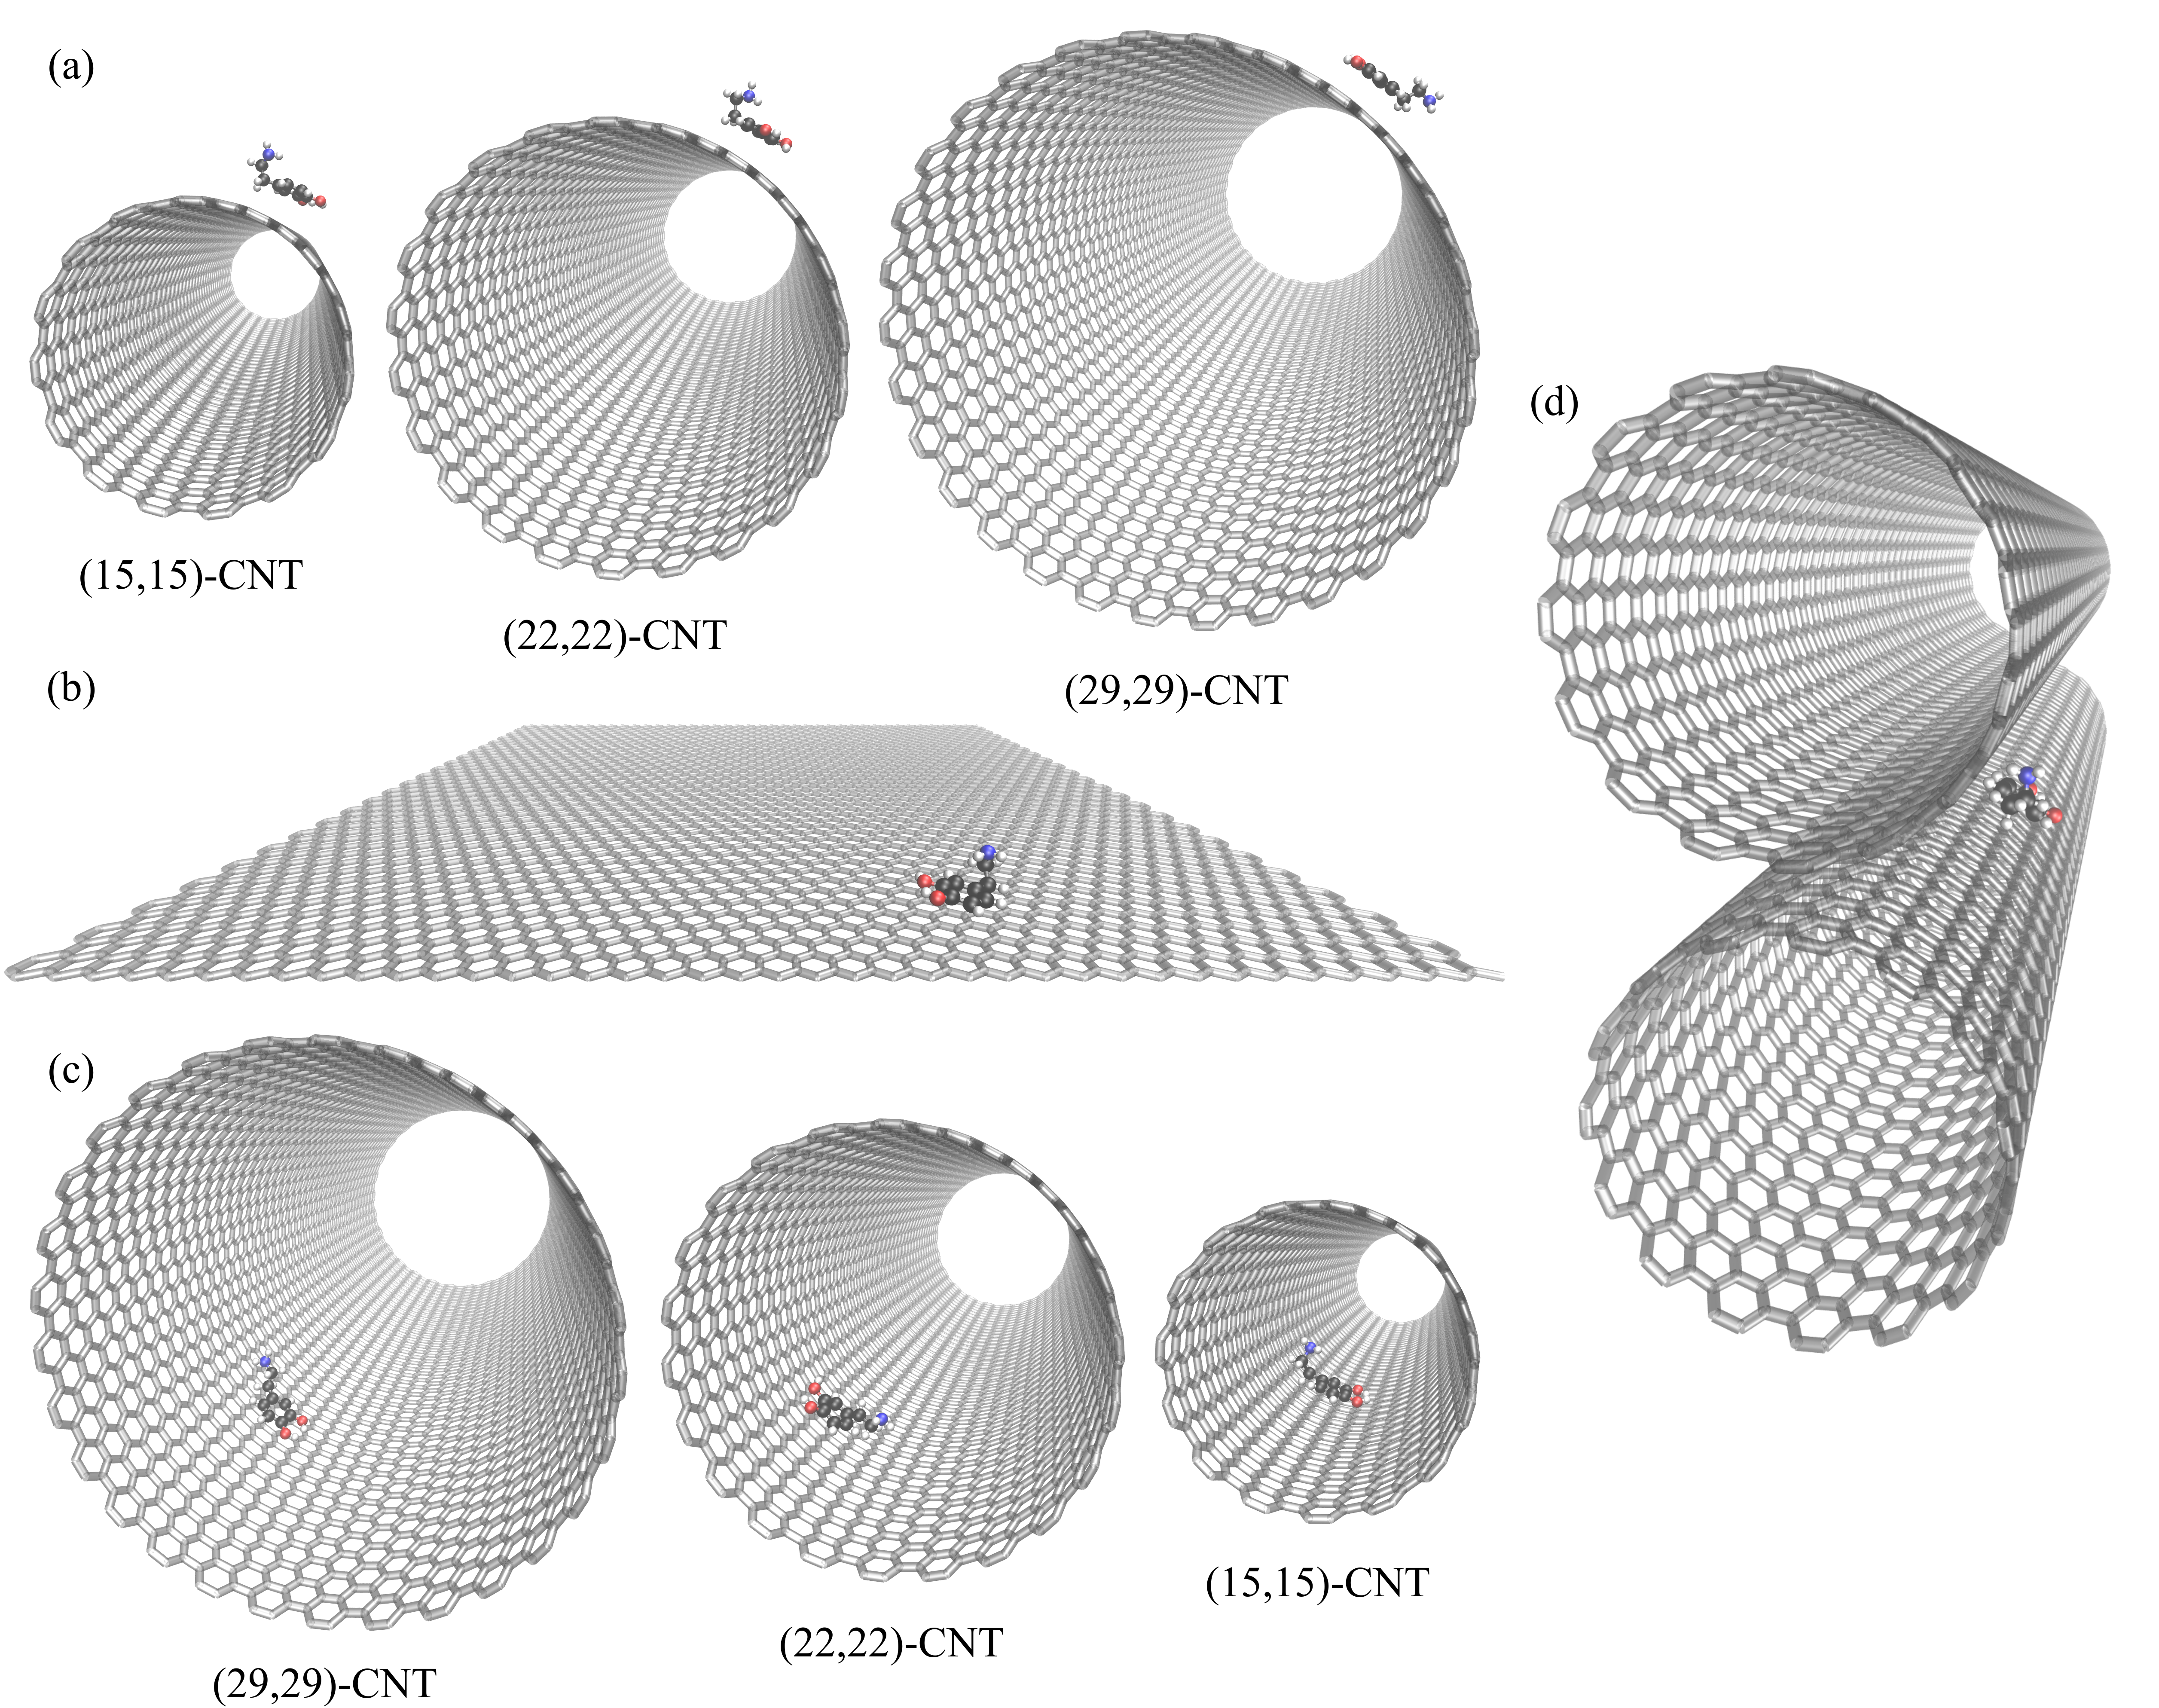
\includegraphics[width=.95\textwidth]{Methods/methods.png}
    \caption{Simulated CNT and graphene surfaces. %MDPI: 1. Is the bold is necessary? Can we delete it? Please confirm. Please also check all figures caption in the main text. 2. please check if the dot should be comma (e.g., 29.29 should be 29,29) %AuthorResponsetoMDPI: Fixed. Removed bolding figure and table headings. 
 DA is shown on (\textbf{a}) the exterior surfaces of CNTs of varying curvatures, (\textbf{b}) flat graphene, and (\textbf{c}) the corresponding CNT interiors. In~(\textbf{d}), DA diffuses along the exterior groove formed by two parallel $(15,15)$-CNT nanotubes. The~dimensions of the CNTs are listed in Table~S1, and~the solvating water molecules were omitted here for visual~clarity.}
    \label{fig:Methods_model_surfaces_CNTs}
\end{figure}




\subsection{DA and DOQ~Adsorbates}

We modeled DA and DOQ atomistically, along with their physiologically relevant protonated counterparts, DAH$^+$ and DOQH$^+$ \cite{Nishihira1997}. A~description of the partial charge assignments can be found in~\cite{Jia2022}. Cl$^-$ ions were added as countercharges for the protonated species. DA and its derivatives contain three key moieties: the side-chain amine, the~aromatic ring, and~an \textit{ortho}-diol or quinone group~\cite{Meiser2013}, see Figure~\ref{fig:Methods_model_adsorbates_moieties}. We also modeled the dynamics of a charge neutral atomic adsorbate with the same molar mass as dopamine (153.18 a.u.), which is referred to as ``adatom(DA)''.

\begin{figure}[H]
    %\centering
{\captionsetup{position=bottom,justification=centering}
    \subfloat[\centering][DA]{\includegraphics[width=.3\textwidth]{Figures/DA_labeling/DA_relabelled.jpg}}
    \subfloat[\centering][DOQ]{\includegraphics[width=.3\textwidth]{Figures/DA_labeling/DOQ_relabelled.jpg}}
}
    \caption{DA and DOQ. The adsorbate structures of DA and DOQ are shown here. The~corresponding protonated species, DAH$^+$ and DOQH$^+$, have an additional hydrogen in their positively charged amine groups. The~C2--C7 vectors (red arrows) are used to define the orientation and tilt of the adsorbates above the carbon~surface.}
    \label{fig:Methods_model_adsorbates_moieties}
\end{figure}

\section{Results and~Discussion}
 


\subsection{Solvated Adsorbate Diffusivities Depend on Surface~Curvature}



Inspired by previous work showing that variations in surface curvature and CNT helicity can alter the diffusional pathways of an atomic adatom on a CNT surface~\cite{Shu2001}, we set out to investigate the motion of DA across a series of solvated CNT surfaces with varying curvatures. The~mean squared displacements (MSDs) of the adsorbates along the CNT axis (MSD$_\parallel$) and around its circumference (MSD$_\perp$) are plotted in Figure~\ref{fig:curvature_dependency_MSD}b as a function of time for DA on seven differently curved armchair CNT surfaces: three on the CNT interior, one on flat graphene, and~three on the CNT exterior. The~1D diffusivities, $D_\perp$ and $D_\parallel$, and~the overall 2D diffusivities, $D$, are listed in Figure~\ref{fig:curvature_dependency_MSD}c. The~diffusion coefficients, $D$, were computed from the MSDs using the Einstein relation,~\cite{Alexiadis2008, ums} as detailed in the~Supplementary Materials. % We revised ''SI'' to ''Supplementary Materials'', please confirm if ithis revision is fine with you. %AuthorResponsetoMDPI: It is fine with us.

\begin{figure}[H]
    %\centering
    \includegraphics[width=\textwidth]{MergedFigs/fig3/output.png}
    \caption{DA diffusion on differently curved carbon surfaces. Results are shown here for the diffusion of DA on the interior (int) and exterior (ext) surfaces of armchair CNTs of varying diameters and flat graphene. (\textbf{a}) The armchair designation \cite{Tomanek2014} refers to the edge morphology of the CNT along the perpendicular direction. %MDPI: Please ensure that permission has been obtained and there is no copyright issue. If copyright is needed, please provide a citation in the following format: “Reprinted/adapted with permission from Ref. [XX]. Copyright year, copyright owner’s name”. More details on “Copyright and Licensing” are available via the following link: https://www.mdpi.com/ethics#10.. %AuthorResponsetoMDPI: Subfigure (a) is our original artwork and is not a reprint from another paper.
 Diffusion on the surface in the same direction as the CNT axis is referred to as parallel ($\parallel$), while that around the circumference of the CNT is denoted as perpendicular ($\perp$). All CNTs presented in this table are 100.698~\AA\ along the periodic $\parallel$ direction, and~the graphene sheet is $98.2419\times97.8420$~\AA$^2$ in size and periodic in two directions along the surface. (\textbf{b}) The MSDs as a function of time are shown in both surface directions: $\perp$ (top panel) and $\parallel$ (bottom panel).\linebreak (\textbf{c}) The diffusion constants $D_{\perp}$, $D_{\parallel}$, and~the overall 2D $D$ values are computed from linearly fitting the MSD curves in (\textbf{b}) using the Einstein relation, Equation~(S4), %MDPI: please confirm this revision. %AuthorResponsetoMDPI: Looks good.
 over~the 4--10 ps range. In~both (\textbf{a},\textbf{b}), the~carbon surface results are organized from most concave to the most~convex. }
    \label{fig:curvature_dependency_MSD}
\end{figure}




The observed diffusion constants are smallest on the convex CNT exterior and largest on the concave CNT interior. The~largest shifts with curvature are seen in the $D_\perp$ values, in~keeping with the direction in which the surface curves. In~addition, a~clear increase is seen in the $D_\perp$ values among the CNT interior results as the concavity increases from $(29,29)$-CNT$_\mathrm{int}$ to $(15,15)$-CNT$_\mathrm{int}$.

{In order to compare the resulting diffusion constants to experimental values, we adjust them to correct for an unphysical system size dependence. This known finite-size \linebreak effect~\cite{Fushiki2003PRE, Yeh2004JPCB, Simonnin2017, Jamali2018JCTC} is discussed in more detail in the Supplementary Materials % We revised ''SI'' to ''Supplementary Materials'', please confirm if ithis revision is fine with you.
 (see Figure~S4 and accompanying text), and~the values of the diffusion constants extrapolated to the infinite system size, $D_{\infty}$, are shown for a subset of the cases in Table~\ref{tab:Tech_boxsize_calibration}. \textls[-25]{In~our simulations, the~extrapolated 2D diffusion coefficient of DA on flat graphene is $1.3~\times~10^{-5}\ \mathrm{cm^2/s}$, while its value ranges from (1.1--2.5) $\times10^{-5}\ \mathrm{cm^2/s}$ for DA on differently curved CNTs. For~comparison, the~3D diffusion coefficient calculated for DA from flow injection experiments is $0.6\times10^{-5}\ \mathrm{cm^2/s}$ \cite{Gerhardt1982}.} }


\begin{table}[H]
\caption[Diffusion coefficients extrapolated to the infinite system sizes.]{Diffusion coefficients extrapolated to the infinite system sizes. %MDPI: Please confirm if the bold should be retained, please check all tables caption. %AuthorResponsetoMDPI: removed bolding.
 For a subset of the carbon surfaces, diffusion constants for the infinite system sizes, $D_\infty$, were extrapolated from a series of differently sized finite simulations. The~extrapolation was done to correct for unphysical effects that arise from the necessarily finite simulation sizes, and~the $D_\infty$ values thus represent the actual diffusivities expected within the larger physical systems. See SI and Figure~S4 for details.}
    %\centering
    \footnotesize
    \begin{tabularx}{\textwidth}{CCCCC}
    \toprule
    \textbf{Adsorbate} & \textbf{Carbon Surfaces} & \boldmath{$D_{\infty, \perp}$} \textbf{(}\boldmath{$\times10^{-5}$ \textbf{cm}$^2$}\textbf{/s)} & \boldmath{$D_{\infty, \parallel}$} \textbf{(}\boldmath{$\times10^{-5}$ \textbf{cm}$^2$}\textbf{/s)} & \boldmath{$D_\infty$ ($\times10^{-5}$} \textbf{cm}\boldmath{$^2$}\textbf{/s})\\
    \midrule
    
        \multirow{3}{*}{DA}         &   $(15,15)$-CNT$_\mathrm{int}$   &   $3.50\pm0.15$   &   $1.41\pm0.19$  &   $2.45\pm0.13$\\
                                    &   Flat Graphene   &   $1.27\pm0.07$   &   $1.22\pm0.10$  &   $1.24\pm0.06$\\
                                    &   $(15,15)$-CNT$_\mathrm{ext}$   &   $1.17\pm0.02$   &   $1.06\pm0.05$  &   $1.12\pm0.03$\\
    \bottomrule
    \end{tabularx}
    \label{tab:Tech_boxsize_calibration}
\end{table}









{\bf{Curvature dependence is observed for DA, DAH$^+$, DOQ, and~DOQH$^+$.}}
Table~\ref{tab:Results_curvature_derivatives}\linebreak presents the diffusion constants obtained for these four species on both the interior and exterior surfaces of $(15,15)$-CNT, along with the flat graphene results. From~these measurements, we find that the curvature-dependence is similar across all four~species.

\begin{table}[H]
\caption{2D diffusion coefficients of DA, DOQ, and~their protonated counterparts. The values of the overall 2D diffusion constant, $D$, were calculated from the MSDs of the adsorbates on the interior of the armchair $(15,15)$-CNT, flat graphene, and~the exterior of the armchair $(15,15)$-CNT. Finite system size results are shown here as calculated within the $\approx$100~\AA\ long~systems.}
    \footnotesize
    %\centering
    \begin{tabularx}{\textwidth}{m{3cm}CCCC}
        \toprule
        \multirow{2}{*}\textbf{{\boldmath{$D$} (\boldmath{$\times10^{-5}$} \textbf{cm}\boldmath{$^2$}\textbf{/s})}\vspace{-10pt}}& \includegraphics[scale=0.3]{Figures/vertical_distn/DA.jpg} & \includegraphics[scale=0.3]{Figures/vertical_distn/DAH.jpg} & \includegraphics[scale=0.3]{Figures/vertical_distn/DOQ.jpg} & \includegraphics[scale=0.3]{Figures/vertical_distn/DOQH.jpg} \\
        & \textbf{DA} & \textbf{DAH}\boldmath{$^+$} & \textbf{DOQ} & \textbf{DOQH}\boldmath{$^+$} \\
        \midrule
        $(15,15)$-CNT$_\mathrm{int}$ & $3.34    \pm 0.26$ & $3.24   \pm 0.21$   &   $3.72   \pm 0.29$   &   $3.65   \pm 0.35$ \\
        Graphene        & $1.92    \pm 0.07$ & $1.74   \pm 0.07$   &   $2.29   \pm 0.16$   &   $1.95   \pm 0.14$ \\
        $(15,15)$-CNT$_\mathrm{ext}$ & $1.30    \pm 0.04$ & $1.20   \pm 0.06$   &   $1.53   \pm 0.10$   &   $1.37   \pm 0.05$ \\
        \bottomrule
    \end{tabularx}
    \label{tab:Results_curvature_derivatives}
\end{table}

In addition, across all three curvatures we find that the protonated species, DAH$^+$ and DOQH$^+$, diffuse more slowly than their neutral counterparts, DAH and DOQ, while the oxidized species, DOQ and DOQH$^+$, diffuse more rapidly than their reduced counterparts, DA and DAH$^+$. These trends were previously observed on flat graphene~\cite{Jia2022} and can be readily explained by differences in the interactions of each species with the solvating water molecules: the positively charged species have increased interactions with the polar solvent, while the oxidized species have reduced interactions with the solvent---their quinone moieities are only able to act as hydrogen bond acceptors, as~compared to the reduced diol moieties, which can act as both hydrogen bond donors and acceptors. Increased attractions with the solvent will increase the adsorbate's effective hydrodynamic radius, $R_{\rm H}$, which is inversely related to the diffusion constant, $D$, of~a solvated sphere in nonturbulent flow via the Stokes--Einstein equation~\cite{nanofluidics}:
$D=\dfrac{k_\mathrm{B}T}{c\pi\eta R_\mathrm{H}}$, where $k_\mathrm{B}$ is the Boltzmann constant, $T$ is temperature, $\eta$ is solvent viscosity, and~$c$ is a constant that describes the boundary conditions at the solvent-sphere interface. The~Stokes--Einstein equation cannot be rigorously applied here for these partially solvated, small molecular adsorbates; however, it qualitatively explains the observed~trends. 

\newpage

Our simulation results show that DA diffusion clearly depends on placement on the inner or outer surface of the CNT, with~enhanced motion on the CNT interior. Overall, this observed curvature dependence is consistent with the general trends observed previously for an atomic adatom~\cite{Shu2001}. 


\subsection{Dependence Does Not Arise from Curvature-Induced Shifts in Surface~Roughness}

In the case of the previously studied atomic adatom, the~observed reduction of diffusion barriers for the adatom on a surface with negative curvature (the CNT interior) resulted from the smoothing of the carbon energy surface as it changes from convex to flat to concave~\cite{Shu2001}. However, it is not clear how this effect functions for a molecular adsorbate such as DA, which is larger than the underlying hexagonal carbon structure, flexible, and~asymmetric in shape with an uneven charge distribution. In~addition, the~role of solvent was not considered in the prior work and may mitigate the influence of surface energy roughness. In~this section, we probe the role of surface roughness in this system by investigating how the lateral distributions of these adsorbates depend on curvature, how their diffusivities depend on CNT helicity, and~how their diffusivities depend on curvature in the absence of~solvent.



{\bf Lateral distributions of molecular adsorbates are similar across curvatures.}  %MDPI: Please confirm if the bold should be retained %AuthorResponsetoMDPI: bold should be retained.
In\linebreak Figure~\ref{fig:Conf_lateral_DA}, we plot the lateral distributions for the adatom(DA), DA, and~its moieties on three differently curved surfaces: the exterior of a $(15,15)$-CNT nanotube, flat graphene, and~the interior of a $(15,15)$-CNT nanotube. By~comparing these distributions to the underlying hexagonal aromatic ring pattern of the carbon surfaces, we can observe how curvature-induced differences in the energy surface roughness influence the placement of these atomic and molecular~adsorbates.



First, we consider the lateral distributions of adatom(DA), an~atomic adatom with the same mass as DA. Shown in the first row of Figure~\ref{fig:Conf_lateral_DA}, these distributions clearly display the characteristic hexagonal pattern that corresponds to the centers of the honeycomb structure of the aromatic carbon surface. As~the surface curvature changes from convex to concave, the~lateral distribution of adatom(DA) gradually becomes more uniform, as~expected from the previously noted smoothing of the surface energy as the curvature becomes more negative~\cite{Shu2001}. Despite the presence of solvating waters in our simulation, the~dependence of adatom(DA)'s lateral distribution on the underlying carbon structure and its curvature~persists.


In contrast, the~lateral distributions of DA's COM and that of its constituent moieties, as~shown in the next four rows of Figure~\ref{fig:Conf_lateral_DA}, display almost no dependence on the underlying hexagonal carbon structure and we see no clear trend in the distributions with curvature. This lack of structuring and curvature dependence suggests that the underlying surface energy roughness is not a dominant factor in determining the lateral placement of DA, which extends spatially over a region larger than the hexagonal lattice spacing of the underlying carbon~surface. 



{\bf Diffusion coefficients for zigzag and armchair CNTs are indistinguishable.} %MDPI: Please confirm if the bold should be retained %AuthorResponsetoMDPI: bold should be retained.
Helicity-dependent diffusion of atomic adsorbates on CNT surfaces has been previously observed in simulations, where different diffusive pathways were observed on armchair and zigzag CNT surfaces due to the surface energy landscapes that emerged upon curving graphene in different directions~\cite{Wu2006, Shu2001}. To~probe this effect for our solvated system, we simulated the diffusion of both DA and adatom(DA) on the interior and exterior surfaces of highly curved armchair and zigzag CNTs. Figure~\ref{fig:armchair-zigzag} shows the two CNT structures with 10~\AA\ radii ($(15,15)$-CNT and $(0,26)$-CNT) as well as the $D_{\perp}$, $D_{\parallel}$, and~2D $D$ values obtained from these simulations. The~corresponding results on flat graphene are also shown in each case for~comparison.

\begin{figure}[H]
    %\centering
    \includegraphics[width=0.9\textwidth]{Figures/moieties_com_distn/DA_lateral_moieties_distributions_full.png}
    \caption{Lateral distributions of adatom(DA) and DA above the CNT and graphene surfaces. The plots show the distribution densities of the adsorbates above the carbon surface. From~left to right, the~columns show the distributions on the exterior surface of $(15,15)$-CNT, on~flat graphene, and~on the interior surface of $(15,15)$-CNT, as~indicated with the cartoon images above each column. From~top to bottom, the~rows show the results for adatom(DA) (an atomic adatom with the mass of DA), the~COM of DA, and~the three COMs of the red-circled DA moieties. The~projected COM coordinates are binned with a spatial resolution of $0.1\times0.1$ \AA$^2$ and wrapped into 4 unit cells, which are separated by the dashed~lines.}
    \label{fig:Conf_lateral_DA}
\end{figure}





We found no significant difference between the armchair and zigzag diffusion constants in our simulations for either the atomic or molecular DA adsorbates. This result is expected for DA itself, given the insensitivity of its lateral distribution to the underlying hexagonal structure in  Figure~\ref{fig:Conf_lateral_DA}. The~shift in the lateral distribution for adatom(DA) with curvature, however, suggests that differences between zigzag and armchair diffusivities are possible within our system. Even so, the~results for the two cases are statistically indistinguishable, perhaps due to the dominant influence of surface hydration on adsorbate dynamics in these systems which we found in our prior work on flat graphene~\cite{Jia2022}. 

\begin{figure}[H]
    \footnotesize
    %\centering
    \includegraphics[width=.4\textwidth]{Methods/chirality/fig_3.png}\\
    \begin{tabular}{cc|cc|c}
        \toprule
        Adsorbate &Carbon Surfaces & $D_\perp$ ($\times10^{-5}$ cm$^2$/s) & $D_\parallel$ ($\times10^{-5}$ cm$^2$/s) & $D$ ($\times10^{-5}$ cm$^2$/s) \\
        \midrule
        \multirow{6}{*}{DA} &	$(15,15)$-CNT$_\mathrm{int}$ &   $4.34   \pm 0.26$   &   $2.34   \pm 0.32$  &   $3.34   \pm 0.26$\\
                                    &	Graphene              &   $1.92   \pm 0.12$   &   $1.92   \pm 0.13$  &   $1.92   \pm 0.07$\\
                                    &	$(15,15)$-CNT$_\mathrm{ext}$ &   $1.21   \pm 0.06$   &   $1.39   \pm 0.08$  &   $1.30   \pm 0.04$\\
                                    \cmidrule{2-5}
                                    &   $(0,26)$-CNT$_\mathrm{int}$ &    $4.56   \pm 0.44$   &   $2.39   \pm 0.17$  &   $3.48 \pm 0.20 $ \\
                                    &   Graphene              &    $1.92   \pm 0.13$   &   $1.92   \pm 0.12$  &   $1.92 \pm 0.07 $ \\
                                    &   $(0,26)$-CNT$_\mathrm{ext}$ &    $1.20    \pm 0.10$    &   $1.42   \pm 0.11$  &   $1.31	\pm	0.08$ \\
        \midrule
        \multirow{6}{*}{Adatom(DA)} &	$(15,15)$-CNT$_\mathrm{int}$ &   $8.08   \pm   0.99$   &   $5.14   \pm 0.51$ &   $6.61   \pm 0.52$ \\
                                    &	Graphene              &   $4.59	  \pm	0.32$	&	$4.71	\pm	0.31$ &   $4.65   \pm 0.29$ \\
                                    &	$(15,15)$-CNT$_\mathrm{ext}$ &   $2.95	  \pm	0.21$	&	$3.12	\pm	0.27$ &   $3.03   \pm 0.15$ \\
                                    \cmidrule{2-5}
                                    &   $(0,26)$-CNT$_\mathrm{int}$ &   $8.04   \pm 0.35$   &   $4.71   \pm 0.46$   &   $6.38   \pm 0.32$ \\
                                    &   Graphene              &  $4.71   \pm 0.31$   &  $4.59   \pm 0.32$   &    $4.65   \pm 0.29$ \\
                                    &   $(0,26)$-CNT$_\mathrm{ext}$ &   $2.96   \pm 0.20$   &   $3.19   \pm 0.16$   &   $3.04   \pm 0.15$ \\
        \bottomrule
    \end{tabular}
    \caption{Diffusion coefficients of DA and adatom(DA) on armchair and zigzag CNTs. Armchair and zigzag CNTs are two conformations which describe the carbon atom arrangements along the perpendicular direction%MDPI: Please ensure that permission has been obtained and there is no copyright issue. If copyright is needed, please provide a citation in the following format: “Reprinted/adapted with permission from Ref. [XX]. Copyright year, copyright owner’s name”. More details on “Copyright and Licensing” are available via the following link: https://www.mdpi.com/ethics#10.. %AuthorResponsetoMDPI: the top subfigure is our original artwork and is not a reproduction of a previous paper.
. The~values of the diffusion constants $D_{\perp}$, $D_{\parallel}$ and~the overall 2D $D$ were calculated from the MSDs of the adsorbates on the different surfaces. The~1D diffusion constants on the flat graphene surface along the direction with the same chirality as each CNT direction were chosen for the comparison. Finite system size results are shown here as calculated within the 100~\AA\ long~systems.} 
    \label{fig:armchair-zigzag}
\end{figure}



{\bf Curvature dependence of $D$ disappears in the absence of solvent.}  %MDPI: Please confirm if the bold should be retained %AuthorResponsetoMDPI: the bold should be retained.
The negligible influence of the carbon surface's hexagonal patterning on DA's lateral distributions in Figure~\ref{fig:Conf_lateral_DA} suggests that the differences in $D$ between the CNT surfaces of various curvature in Figure~\ref{fig:curvature_dependency_MSD} and Table~\ref{tab:Tech_boxsize_calibration} do not actually arise from curvature-mediated changes to the energetic interactions between the adsorbate and the surface. The~lack of dependence of DA diffusion on CNT helicity in Figure~\ref{fig:armchair-zigzag} supports this~conclusion.  
         
To isolate the adsorbate--surface interactions and further probe this dependence directly, in~Figure~\ref{fig:D-nosolvent} we plot MSD$_{\parallel}$ and MSD$_{\perp}$ for DA and DOQ on the carbon surfaces in the absence of solvent. Only the neutral species are simulated due to the lack of charge balance under vacuum conditions. The~average MSD results for the adsorbates on flat graphene and on the interior and exterior of the $(15,15)$-CNT at the vacuum interface are shown plotted with lines, while the noise on each measurement is indicated by the shaded~regions. 


      
The resulting curves are not linear over the time regime plotted, indicating that inertial motion lasts for much longer times at the carbon:vacuum interface than at the carbon:water interface. Since the simulations do not allow for carbon surface fluctuations, which would be expected to significantly reduce the timescale of inertial motion decay in the absence of solvent, these MSD curves are only useful as a way to isolate the direct interactions between the adsorbate and the different carbon surface architectures and test their influence on adsorbate~diffusion.
      
\begin{figure}[H]
    %\centering
    \includegraphics[width=0.6\textwidth]{Figures/MSD_trajs_no_solvent/msd_trajs.png}
    \caption{MSDs of DA and DOQ on differently curved carbon:vacuum surfaces. The top and bottom panels show the MSDs as a function of time along two surface directions, $\parallel$ and $\perp$, on~graphene and on the interior and exterior of the $(15,15)$-CNT. The~left and right panels display the results for adsorbates DA and DOQ, respectively. 
    The lines show the average MSD values, while the shaded regions show the standard deviation in that value across ten trials, with~red shading for $(15,15)$-CNT$_{\rm int}$, green shading for flat graphene, and~blue shading for $(15,15)$-CNT$_{\rm ext}$.}
    \label{fig:D-nosolvent}
\end{figure}

The results within each panel show significant overlap of the shaded regions and no observable curvature dependence. In~addition, the~difference between the diffusivities of DA and DOQ disappears, as~expected from our conclusions above regarding the importance of solvent and the effective $R_{\rm H}$ in determining the relative diffusivities of DA, DOQ, and~their protonated species~\cite{Jia2022}. Finally, even the MSD$_{\perp}$ and MSD$_{\parallel}$ curves appear identical, indicating that the differences observed in CNT surface diffusion between the axial and perpendicular directions in Figure~\ref{fig:curvature_dependency_MSD} and Table~\ref{tab:Tech_boxsize_calibration} are also attributable to solvent~effects.

Taken together, these results suggest that the curvature dependence that we observe in the diffusion constants for adsorbed DA and DOQ at the carbon:water surface do not actually arise from curvature-induced changes in the energy surface roughness, as~was the case in the prior work on an unsolvated atomic adatom~\cite{Shu2001}. Instead, we conclude that the curvature-dependence of these molecular adsorbates' diffusivities arises from a more complex interplay of surface curvature and surface~solvation. 

\subsection{Adsorbate Structure Depends on Curvature, Charge, and~Solvation}

In this section, we investigate in detail the adsorbate's configuration on the surface and its dependence on curvature, charge, and~solvation. First, we examine the vertical placement of DA and DOQ and its constituent moieties above the different carbon surfaces; in~particular, we examine the various configurations available to the amine group. Then, we consider the tilt angle of the aromatic ring above the surface and the adsorbate's orientational alignment with the CNT axis. Finally, we consider how the differently curved surfaces shift the number of water molecules in the first solvation shell around the adsorbate, which will influence the effective hydrodynamic radius, $R_{\rm H}$, and,~therefore, the~diffusivity.



{\bf The distance of the adsorbate above the surface depends on curvature, charge, and~solvation.} % MDPI: Please confirm if the bold should be retained %AuthorResponsetoMDPI: the bold should be retained.
The vertical distance, $d$, is defined as the distance between the COM of a moiety and its closest point on the carbon surface. Figure~\ref{fig:Conf_vertical_derivatives} displays the vertical distributions for the aromatic ring (left column), the~diol/quinone (middle column), and~the amine group (right column) on the three surfaces. DA and DOQ distributions are shown at both the carbon:water and carbon:vacuum interfaces, while DAH$^+$ and DOQH$^+$ distributions are only shown at the carbon:water~interface. 

\begin{figure}[H]
    %\centering
    \includegraphics[width=0.9\textwidth]{Appendices/derivatives_vertical/output.png}
    \caption{Vertical distributions of DA and DOQ moieties at the carbon:water and carbon:vacuum interfaces. From left to right, three columns show the vertical distributions of the aromatic ring, the~diol/quinone moiety, and~the amine group, respectively, with~$d$ representing the distance between that moiety's COM and the closest point on the surface. From~top to bottom, the~six rows correspond to DA, DA in vacuum, DOQ, DOQ in vacuum, DAH$^+$, and~DOQH$^+$. Colored curves within each subplot indicate the distributions at the flat graphene or the interior and exterior $(15,15)$-CNT~surfaces.}
    \label{fig:Conf_vertical_derivatives}
\end{figure}
    
In the left column of Figure~\ref{fig:Conf_vertical_derivatives}, the~position of the aromatic ring for all solvated species shifts slightly away from the surface as its curvature changes from convex to flat to concave. Due to the ring's structural rigidity, its COM can get closer to the surface when adsorbed on the convex exterior of the CNT than when adsorbed to its concave interior, where interactions with the inward-curving walls shift the center of the ring slightly away from its optimal distance on the flat surface. Interestingly, for~the two cases of DA and DOQ at the carbon:vacuum surface, the~aromatic ring distributions for both the exterior and interior CNT surfaces shift slightly to the right, as~compared to the solvated cases. This shift away from the surface indicates the importance of solvation in determining the optimal vertical position for the CNT-adsorbed aromatic~rings.
  
In contrast, the~diol/quinone moiety distributions in the middle column of Figure~\ref{fig:Conf_vertical_derivatives} display no shift with curvature, although~the peak narrows slightly in all cases as the curvature of the carbon surface changes from convex to flat to concave. The~invariance of these peaks, coupled with their location on the edge of the aromatic ring, provide further evidence that the shift in aromatic ring placement with curvature reflects constraints on the optimal surface ring distance due to the curved surface~geometry.
  
Finally, in~the right column of Figure~\ref{fig:Conf_vertical_derivatives}, we plot the vertical distributions of the amine tail, which is tethered to the aromatic ring through rotatable bonds and can thus adopt a variety of configurations. Our prior work on flat graphene~\cite{Jia2022} demonstrated that the vertical distribution of the amine group is sensitive to its protonation state, as~the positively charged DAH$^+$ and DOQH$^+$ amines can form additional hydrogen bonds with the bulk phase water molecules. These prior observations showed that the neutral amine vertical distributions have three peaks and span a range of about 3--7 \AA~ from the surface, while the positively charged amines have a narrower distribution around a single peak at $\approx$6~\AA\ from the surface. Similar overall distributions are seen for the CNT exterior and interior surfaces, with~a broad, three-peaked distribution for the neutral species and a narrower distribution further from the surface for the charged amines. However, as~the curvature changes from the exterior to flat graphene to the interior, the~amine distributions are altered, especially for the CNT interior. In~addition, we find that the distributions shift closer to the surface for both DA and DOQ at the carbon:vacuum interface as compared to their corresponding distributions at the carbon:water~interface. 



{\bf Amine configurations are highly variable and display significant curvature dependence.}  %MDPI: Please confirm if the bold should be retained %AuthorResponsetoMDPI: the bold should be retained.
Given the complex variation observed in the amine vertical distributions, in \linebreak Figure~\ref{fig:Conf_vertical_DAconf}, we investigate in more detail these distributions for DA at the carbon:water interface. The~three peaks for the CNT$_{\rm ext}$, flat graphene, and~CNT$_{\rm int}$ distributions have been marked with letters in Figure~\ref{fig:Conf_vertical_DAconf}a, their positions are listed in the table shown in Figure~\ref{fig:Conf_vertical_DAconf}b, and~a sample configuration at the characteristic distance within each peak is shown in Figure~\ref{fig:Conf_vertical_DAconf}c. 



   
The peaks closest to the surface in Figure~\ref{fig:Conf_vertical_DAconf}a\emph{(i, iv, vii)} correspond to configurations in which the amine group is in close contact with the surface. These first amine distribution peaks are observed at 3.1--3.7~\AA\ (see Figure~\ref{fig:Conf_vertical_DAconf}b) on all three surfaces, which is close to the sum of the van der Waals (vdW) radii, 3.27~\AA, of~a carbon with a nitrogen in the OPLS-AA force field~\cite{OPLS-AA}. The~amine groups in these configurations are closest to the water molecules in the first layer near the surface, as~can be seen in the corresponding sample structures in Figure~\ref{fig:Conf_vertical_DAconf}c. The~first and the second peaks in the density profile of water are observed at $\approx$3.3~\AA\ and $\approx$6.2~\AA, respectively (see Figure~S5). The~second set of peaks in the amine distribution \textit{(ii, v, viii)} %MDPI: please check if it should be subfigure citation, please check all format like this . %AuthorResponsetoMDPI: these should remain as is.
 are observed at 4.2--5.2 \AA. The~amine groups in these configurations are therefore likely to form hydrogen bonds with both the first and second layers of water molecules, as~shown in the sample structures in Figure~\ref{fig:Conf_vertical_DAconf}c. Last, the~third set of peaks \textit{(iii, vi, ix)} are seen at 5.6--5.9 \AA, which is closest to the water molecules in the second layer. The~sample configurations for these peaks in Figure~\ref{fig:Conf_vertical_DAconf}c show the amine tail stretching up toward the bulk~water.
   
Although the presence of these three peaks persist across the curvatures, their locations shift with curvature, as~can be seen in Figure~\ref{fig:Conf_vertical_DAconf}a. When the curvature changes from convex (purple) to flat (teal), all three peaks shift rightwards. When the curvature changes from flat to concave (yellow), these three peaks shift back toward the left but~to a lesser~degree.  
    
To understand the trend in the peak closest to the surface, we consider the three structures shown on the left in Figure~\ref{fig:Conf_vertical_DAconf}c. ``Tentlike'' configurations similar to \textit{(i)} are more likely on the convex surface, where the amine group reaches down toward the carbon surface. Even though the center of the aromatic ring is slightly tilted away from the surface, it remains closer to the surface than it would in a similar configuration on a flat or concave surface. The~position of the amine as it points down toward the surface corresponds to the leftmost peak in Figure~\ref{fig:Conf_vertical_DAconf}a, at~3.19 \AA. The~structures \textit{(iv)} and \textit{(vii)} also contain amines quite close to the surface, but~given the mismatch between the surface curvature and the tentlike structures of \textit{(i)}, they are not able to get as close, showing a peak distance of 3.68 \AA\ on the flat graphene surface and of 3.57 \AA\ on the convex surface (see Figure~\ref{fig:Conf_vertical_DAconf}b). 

\begin{figure}[H]
  %\centering
  \includegraphics[width=.7\textwidth]{MergedFigs/fig8/output.png}
\caption{Vertical distributions and configurations of DA at the carbon:water interface. Panel (\textbf{a}) shows the vertical distributions of the amine group of DA on flat graphene and on the exterior and interior of a $(15,15)$-CNT. The~three peaks in each distribution are labeled and correspond to the distances shown in panel (\textbf{b}) and the sample conformations shown in panel (\textbf{c}). Peak positions in (\textbf{b}) were obtained from curve-fitting using Gaussian functions. In~panel (\textbf{c}), only water molecules within 3~\AA\ radius of the nitrogen in the amine group are~displayed.}
\label{fig:Conf_vertical_DAconf}
\end{figure}
   
For the middle peaks, $(ii, v, viii)$, represented by the corresponding structures in the middle column of Figure~\ref{fig:Conf_vertical_DAconf}c, the~leftward shift is even stronger for DA on the convex surface \textit{(ii)} and represents another version of the ``tentlike'' structures---one with the same tilted aromatic ring but~with the amine group pointing back toward the solvent as in structure $(ii)$ in Figure~\ref{fig:Conf_vertical_DAconf}c. In~the next section, we discuss the distributions of these aromatic tilt angles and their curvature dependence. On~the flat and concave surfaces, the~middle peak corresponds to structures where aromatic ring is parallel to the surface and the amine group is rotated away from the surface by one carbon bond in the linker, as~in structures \textit{(v)} \mbox{and \textit{(viii)}.}
  
The third peak from the surface represents the most probably configuration for all curvatures. In~these structures, the~two linker bonds that connect the plane of the aromatic ring to the amine group are both oriented to extend the amine out away from the surface (see structures $(iii, vi, ix)$ in Figure~\ref{fig:Conf_vertical_DAconf}c). The~location of this third peak displays the smallest curvature dependency, as~can be seen in the relatively small range in the most probable distances listed in Figure~\ref{fig:Conf_vertical_DAconf}b, third column. Although~the structures shown in Figure~\ref{fig:Conf_vertical_DAconf}c only include the neutral DA species, this third peak is the only one observed for the positively charged species, DAH$^+$ and DOQH$^+$ (see the last two rows of Figure~\ref{fig:Conf_vertical_derivatives}, right-most column). This result indicates that, when protonated, the~amine group remains fully extended into the solvent for all curvatures, similar to structures $(iii, vi, ix)$. These structures also aid in the interpretation of the amine distributions for DA and DOQ at the carbon:vacuum interface in Figure~\ref{fig:Conf_vertical_derivatives} as well. As~compared to the same amine distance distributions at the carbon:water interface, the~peak locations remain unchanged, but~the relative peak heights shift, indicating that configurations with the amine extending away from the surface are significantly less probable in the absence of~solvent.



{\bf The aromatic ring's tilt angle above the surface depends on curvature, charge, and solvation.} %MDPI: Please confirm if the bold should be retained %AuthorResponsetoMDPI: the bold should be retained.
The distributions of the tilt angle between the aromatic ring and the surface are shown in Figure~\ref{fig:Conf_DA_tilt} for DA on differently curved carbon surfaces at both the carbon:water (Figure~\ref{fig:Conf_DA_tilt}c) and carbon:vacuum (Figure~\ref{fig:Conf_DA_tilt}d) interfaces. In~addition, the~tilt distributions of DA, DOQ, and~their protonated species are shown for flat graphene at the aqueous interface in Figure~\ref{fig:Conf_DA_tilt}e.

\begin{figure}[H]
    %\centering
    \includegraphics[width=\textwidth]{Figures/phi_output.png}
    \caption{Tilt angle distributions of DA and other adsorbates on differently curved and solvated CNT and graphene surfaces. The tilt angle $\phi$ is defined as shown in (\textbf{a},\textbf{b}) between the C2--C7 vector (blue arrows) and a vector tangent to the surface at the midpoint of the C2--C7 vector (red arrows). $\phi$ distributions for DA on differently curved surfaces, plotted as histograms with a binwidth of 0.36$^\circ$, are shown in (\textbf{c}) at the carbon:water interface and in (\textbf{d}) at the carbon:vacuum interface. The~results for DA, DOQ, and~their protonated counterparts are shown in (\textbf{e}) on solvated flat~graphene. }
    \label{fig:Conf_DA_tilt}
\end{figure}
    
When adsorbed on all carbon surfaces, DA primarily adopts configurations in which its aromatic ring is parallel to the surface, as~seen from the dominant peak, which is close to $\phi=0^{\circ}$ in all cases. This configuration maximizes the $\pi$--$\pi$ interactions and is seen in most of the structures shown in Figure~\ref{fig:Conf_vertical_DAconf}c. However, a~second, asymmetric peak is observed in a subset of the cases at $\phi\approx 15^{\circ}$ and corresponds to the tentlike configurations seen in structures \textit{(i)} and \textit{(ii)} in Figure~\ref{fig:Conf_vertical_DAconf}c. The~relative probability of these two tilt angles clearly depends on the surface curvature---the peak at $\phi\approx 0^{\circ}$ is strongest on the most concave surface, whereas the peak at $\phi\approx 15^{\circ}$ is strongest on the most convex~surface.

The tilt angle distributions also display a clear dependence on charge, as~can be seen on solvated flat graphene in Figure~\ref{fig:Conf_DA_tilt}e, where there is substantial probability around $\phi\approx 15^{\circ}$ for DA and DOQ but~no such density for DAH$^+$ and DOQH$^+$. From~the amine group distributions for these positively charged species in Figure~\ref{fig:Conf_vertical_derivatives}, we know that they adopt configurations in which the amine group stretches out into the bulk water, which precludes the more tilted tentlike structures like \textit{(i)} and \textit{(ii)} in Figure~\ref{fig:Conf_vertical_DAconf}c.
    
The tilt angle distribution also depends on solvation. As~can be seen in Figure~\ref{fig:Conf_DA_tilt}d, the~curvature-dependence observed at the carbon:water surface is also present at the carbon:vacuum surface. However, the~population of the tilted configuration increases in all cases, which corresponds well to the shift in the amine distance distribution to values that are closer to the surface for the carbon:vacuum surfaces in Figure~\ref{fig:Conf_vertical_derivatives}. Similar results were obtained for DOQ at the carbon:vacuum interface, see Figure~S6a.


 
{\bf Adsorbate alignment with CNT axis also depends on curvature and solvation.} %MDPI: Please confirm if the bold should be retained %AuthorResponsetoMDPI: the bold should be retained.
In Figure~\ref{fig:theta_distn}, the~orientational alignment of DA with the axis of the CNT, as~defined by $\theta$ in Figure~\ref{fig:theta_distn}a,b, is shown on differently curved carbon surfaces at the carbon:water interface (Figure~\ref{fig:theta_distn}c) and at the carbon:vacuum interface (Figure~\ref{fig:theta_distn}d). The~$\theta$ distributions of DA, DOQ, and~their protonated species are also shown for flat graphene at the aqueous interface in Figure~\ref{fig:theta_distn}e.
\vspace{-6pt}

\begin{figure}[H]
    %\centering
    \includegraphics[width=\textwidth]{Figures/theta_output.png}
    \caption{Orientational alignment of DA and other adsorbates with the CNT axis direction on differently curved and solvated CNT and graphene surfaces. The orientational angle, $\theta$, is defined as the angle between the C2--C7 vector (blue arrows) and the CNT axis direction (red arrows), as~shown in (\textbf{a},\textbf{b}). $\theta$ distributions of DA on differently curved surfaces, plotted as histograms with a binwidth of  3.6$^\circ$, are shown in (\textbf{c}) for the carbon:water interface and in (\textbf{d}) for the carbon:vacuum interface. The~same results for DA, DOQ, and~their protonated counterparts are shown \linebreak in (\textbf{e}) on solvated flat graphene. $\theta$ has a range of $[0,180^\circ]$; however, the results are wrapped so that $p(\theta) = p(180^\circ-\theta)$, for~all $\theta>90^\circ$, due to the symmetry of the~system.}
    \label{fig:theta_distn}
\end{figure}

At the carbon:water interface, the~$\theta$ distribution of DA is uniform on flat graphene and on the exterior of the CNTs, as~can be seen in Figure~\ref{fig:theta_distn}c. In~addition, charge does not seem to influence this orientation for the solvated flat graphene case shown in Figure~\ref{fig:theta_distn}e. Even the flat graphene case at the carbon:vacuum interface in Figure~\ref{fig:theta_distn}d shows no change in the probability with $\theta$. This invariance of the probability of a given $\theta$ orientation on flat graphene is to be expected, given the lack of curvature to break the symmetries present in the flat graphene case as well as the lack of significant lateral distribution patterning in Figure~\ref{fig:Conf_lateral_DA}.
    
In contrast, on~the solvated CNT interior in Figure~\ref{fig:theta_distn}c, there is a marked decrease in the orientational probability as $\theta$ approaches $90^{\circ}$, and~the effect becomes more dramatic as the concavity increases. These highly curved interior surfaces favor orientations where the longest axis of DA is oriented along the CNT axis ($\theta=0\pm40^{\circ}$). This orientational preference is linked to the rightward shift in the aromatic ring's vertical distribution as the surface changes from flat to concave, as~shown in Figure~\ref{fig:Conf_vertical_derivatives}a. In~configurations where DA is not aligned with the CNT axis, its interactions with the inward-curving walls will force the center of the ring slightly away from its optimal distance above the surface. The~data obtained from ten trajectories show that, on~the solvated interior of the $(15,15)$-CNT nanotube, where this orientational preference is strongest, the~average vertical distance of the ring's COM for all configurations in which DA is closely aligned with the CNT axis ($|\theta|<5^{\circ}$) is $3.66\pm0.15$~\AA, whereas the average vertical distance for the configurations where DA is perpendicularly aligned to the CNT axis ($85^{\circ}<|\theta|<95^{\circ}$) is $3.90\pm0.17$~\AA.

The $\theta$ distribution is entirely different at the carbon:vacuum interface, however. Orientations aligned with the CNT axis are disfavored on the CNT interior, and~the most favorable orientation on the CNT interior shifts to $\approx$65$^{\circ}$. At~the same time, orientations aligned with the CNT axis are favored on the CNT exterior. Both trends grow stronger with increased curvature, and~the same trends were observed for DOQ at the carbon:vacuum interface (Figure~S6b).

{\bf Adsorbate solvation shell depends on curvature and influences} \boldmath{$R_{\rm H}$}\textbf{.} %MDPI: Please confirm if the bold should be retained %AuthorResponsetoMDPI: the bold should be retained.
 According to the Stokes--Einstein equation, the~diffusion constant, $D\propto (1/R_{\rm H})$, where $R_{\rm H}$ is the effective hydrodynamic radius, which depends on the magnitude of attractions between the diffusing particle and the nearby solvent molecules. In~the case of a particle adsorbed to a surface, solvation is necessarily limited by the presence and geometry of that surface. Although~the Stokes--Einstein relation cannot be directly applied in that situation, it does provide a way to think about the influence of the degree of solvation on diffusion, as~the magnitude of any favorable interactions between the particle and nearby solvent will influence the particle's effective hydrodynamic radius, $R_{\rm H}$. To~investigate this effect, we calculated the number of solvating water molecules within the first water shell around the DA or DOQ atoms for each surface architecture. A~distance of 5~\AA\ was chosen as the cutoff of that first water shell based on the distribution shown in Figure~S5. The~results are shown in Figure~\ref{tab:watershell}a and display a clear trend from fewest solvating waters on the smallest CNT's interior to the most solvating waters on the smallest CNT's exterior---as expected given the geometric constraints of the surface. This trend matches that seen in the diffusion constants on different surface curvatures, as~seen in Figure~\ref{fig:curvature_dependency_MSD}c. To~determine how well this solvation effect can explain the trend in diffusivities, we plotted in Figure~\ref{tab:watershell}b the diffusivities from Figure~\ref{fig:curvature_dependency_MSD}c vs. $(N_{\rm water})^{-1/3}$, where $N_{\rm water}$ is the number of waters within 5~\AA\ of a DA atom, since $D\propto (1/R_{\rm H})$, and~$R_{\rm H}$ is roughly $\propto (N_{\rm water})^{1/3}$. The~correspondence is quite strong, and~this effect is even able to explain the overlapping values seen in the diffusivities even as curvature steadily changes for the CNT exteriors and for the $(22,22)$-CNT$_\mathrm{int}$ and $(29,29)$-CNT$_\mathrm{int}$ cases. Since there is a clear geometric trend across these different diameter CNTs, the~fact that the number of solvating waters is the same implies that a change in the adsorbate structures, as~documented above, must compensate for that change in a way that maintains a similar degree of~solvation.



Overall, we find here that the vertical placement of the adsorbate and its moieties above the carbon surface, as~well as its tilt angle and alignment with the CNT axis depend in a complex manner on curvature, solvation, and~charge. In~addition, the~degree of DA solvation varies with curvature and can explain much of the trend observed as $D$ varies across~curvatures.

\begin{figure}[H]
    %\centering
    \includegraphics[width=\textwidth]{MergedFigs/fig11/output.png}
    \caption{Correspondence between CNT surface, solvating waters, and~$D$. (\textbf{a}) The number of waters in the first solvation shell around DA are calculated across the different surfaces. For~a given water molecule, its distance to DA is the shortest distance between its oxygen atom and any the atoms of DA. Only the water molecules that are on the same side of the surface as DA are counted. $N_\mathrm{water}$ and its statistical errors were computed from 10 trajectories. (\textbf{b}) The diffusion constants, $D$, from~Figure~\ref{fig:curvature_dependency_MSD}c are plotted vs. $N_\mathrm{water}^{-1/3}$ for DA on a range of differently curved surfaces. A~linear fit line is shown here along with the coefficient of determination, $R^2$.}%MDPI: please change hyphen to minus sign %AuthorResponsetoMDPI: Done.
    \label{tab:watershell}
\end{figure}

\subsection{DA Localizes and Diffuses within a CNT~Groove}

Since a pair of aligned CNTs is the simplest multi-CNT structure expected within CNT-based material, we also investigated how DA behaves on a groove surface, both for the solvated and vacuum~cases.



In all the simulations, DA localized to the groove between the two CNTs within 2--8 ns and remained there. Given this strong structural preference, we ran each simulations for at least 5~ns after it found its way to the groove. All results presented in this section were obtained from the portions of the trajectories where DA is within the CNT~groove. 

A typical configuration from a groove simulation is shown in Figure~\ref{fig:Defects_groove_lateral}a, the~lateral distribution of DA is shown in Figure~\ref{fig:Defects_groove_lateral}b, and~the 3D distribution is shown in Figure~\ref{fig:Defects_groove_lateral}c. There is a slight dependence on the underlying hexagonal structure in the lateral density distribution in Figure~\ref{fig:Defects_groove_lateral}b, but~only the axial direction, as~the adsorbate's location around the circumference is determined by the optimal distance from the other CNT surface, as~can be seen in Figure~\ref{fig:Defects_groove_lateral}c. Note that any lateral patterning will depend on the degree to which the neighboring CNTs are in register. There is a clear separation in the 3D density plot between configurations with DA adsorbed to one CNT surface vs. the other. Jumps between the two CNT surfaces are rare in the solvated case ($1.9\pm0.4$~ns$^{-1}$), but~were more frequently for DA adsorbed at the carbon:vacuum interface ($49.2\pm7.4$~ns$^{-1}$). Jump trajectories across both the carbon:water and carbon:vacuum CNT grooves can be seen in Figure~S7.



Figure~\ref{tab:Defects_groove_diffusion}a compares $D_{\parallel}$ and $D_{\perp}$ for DA in the solvated groove to the same values for DA on the exterior of a single $(15,15)$-CNT, since the groove is constructed of two aligned $(15,15)$-CNTs. Results directly obtained from the 100~\AA-length CNT groove system are shown in the top section of the table, while the extrapolation to the infinite CNT groove is shown at the bottom. Importantly, the~observed trends hold for both the finite size results and the infinite size extrapolations. As~expected, $D_{\perp}$ drops to almost zero when DA remains in the groove. In~contrast, DA's diffusivity along the groove, $D_{\parallel}$, is significantly faster than the corresponding axial diffusivity on the exterior surface of a single CNT. We then calculated $N_{\rm water}$ for DA in the groove and found $26\pm3$ waters within 5~\AA. This value is lower than those reported in Figure~\ref{tab:watershell}a for the other surface structures and explains the faster diffusion within the solvated~groove.

\begin{figure}[H]
    %\centering
    \includegraphics[width=0.98\textwidth]{MergedFigs/fig12/output.png}
    \caption{Spatial distributions of DA in a solvated CNT groove. The COM coordinates of DA within a solvated CNT groove formed by two parallel CNT, as~seen in a typical configuration shown in (\textbf{a}), are plotted here in both (\textbf{b}) 2D and (\textbf{c}) 3D. The~CNT groove is constructed of two parallel, 100~\AA\ $(15,15)$-CNTs. In~the 2D distribution plot in (\textbf{b}), locations along the axial direction were wrapped into two unit cells. The~gray dashed circles represent the location of the surface carbon atoms, and~the black dashed line in the middle at $\perp=0$~\AA\ represents the location on the CNT circumference where the distance between the two CNTs is smallest. The~distribution density in region to the left of that dashed line results from configurations where the adsorbate is closest to the CNT on the left, while the density to the right results from configurations where the adsorbate is closest to the CNT on the right. In~the 3D distribution in (\textbf{c}), the~COM coordinates along the axial direction were wrapped into ten unit cells for~plotting. }
    \label{fig:Defects_groove_lateral}
\end{figure}


Interestingly, this trend is reversed for DA's diffusivity in the groove at the carbon:vacuum interface. Figure~\ref{fig:vacuum_msds}b shows the comparison of the axial MSD of DA in the groove to that of DA on other CNT and graphene surfaces, all at the carbon:vacuum interface. Without~solvent, displacement along the groove is reduced as compared to that on any other surface, which can be readily explained by the presence of two variegated surfaces that can impact DA's inertial motion rather than just~one.

The results for the diffusion of all four adsorbate species within the 100~\AA\ CNT groove are shown in Table~\ref{tab:groove_species_diffusivities}. The~previously observed trends between oxidized and reduced species (oxidized diffuses more rapidly) and between protonated and neutral species (neutral diffuses more rapidly) both hold within the groove~architecture.



\begin{table}[H]
\caption{Diffusion coefficients of DA, DOQ, DAH$^+$, and DOQH$^+$ in a solvated CNT groove. The CNT groove results shown here are reported directly from the finite 100~\AA-long CNT simulations. 
    }
    \footnotesize
    %\centering
    \begin{tabularx}{\textwidth}{CCC}
\toprule
    \textbf{Adsorbate}    &   \boldmath{$D_\parallel$} \textbf{(}\boldmath{$\times10^{-5}$} \textbf{cm}\boldmath{$^2$}\textbf{/s}) &   \boldmath{$D_\perp$} \textbf{(}\boldmath{$\times10^{-5}$} \textbf{cm}\boldmath{$^2$}\textbf{/s}) \\
\midrule
DA		&	$1.82	\pm	0.09$	&	$0.02	\pm	0.01$	\\
DOQ		&	$1.98	\pm	0.17$	&	$0.04	\pm	0.03$	\\
DAH$^+$		&	$1.60	\pm	0.10$	&	$0.02	\pm	0.01$	\\
DOQH$^+$		&	$1.63	\pm	0.05$	&	$0.02	\pm	0.00$	\\
\bottomrule
    \end{tabularx}
    \label{tab:groove_species_diffusivities}
\end{table}


\begin{figure}[H]
    \includegraphics[width=0.99\textwidth]{MergedFigs/fig13/output.png}
    \caption{Diffusion coefficients of DA within a CNT groove. The CNT groove is constructed of two 100~\AA\ long, aligned, $(15,15)$-CNTs. (\textbf{a}) Diffusion constants for the solvated CNT groove and a solvated $(15,15)$-CNT$_\mathrm{ext}$ surface are shown here, both from the 100~\AA\ simulation directly (top rows) and from the infinite-system size extrapolation (bottom rows). $D_\parallel$ is the 1D diffusion coefficient for motion along the CNT groove and axis, and~$D_\perp$ is the 1D diffusion coefficient around the CNT circumference. (\textbf{b}) The axial mean squared displacement of DA is plotted for various surfaces at the carbon:vacuum interface. These MSD results are taken directly from simulations done in the vacuum on 100~\AA\ CNTs and $100\times100$~\AA$^2$ graphene.}
    \label{fig:vacuum_msds}
    \label{tab:Defects_groove_diffusion}
\end{figure}


\section{Conclusions}

Overall, we find that DA and DOQ rapidly diffuse on the surface of pristine CNTs, just as they do on the flat graphene surface~\cite{Jia2022}. Diffusion on a single CNT is rapid both along the CNT axis and around its circumference. This observation corresponds to results from Kim~et~al., who developed a continuum model on the \textmu m scale to demonstrate the catalytic activity of the exterior sidewall of individual CNTs. The~model shows evidence that the entire length of the CNT is uniformly accessible to the electrochemically active analytes, which matched their spatially resolved scanning electrochemical microscopy results~\cite{ac2010kim}.  	

At the same time, we find that the adsorbate diffusivity also depends on the CNT curvature. We observed enhanced adsorbate diffusion as the surface changes from convex to flat to concave. Although~this trend is similar to that observed previously for atomic adsorbates on CNT surfaces~\cite{Shu2001, Liu2013}, its origin differs. 
%{\color{red}[Is this still a good description of Liu2013?  And, if so, what does Liu2013 claim is the cause? The origins of the effect in our system differ from Shu2001, but I'm not sure if that's true for Liu2013.]} {\color{blue}[I think Liu2013 still works in this sentence. Liu2013 observed slower gold adatom diffusion on BN-based and SiO2-based graphene, compared to the diffusion just on graphene. They find two reasons: (a) local surface roughness and (b) homogeneous loss of dispersion/van der Waals electronic stability in multilayers. In their discussions of local surface roughness, they mentioned the local curvatures of both convex and concave sites, but not same as what we do here of just either convex or concave surfaces. So I think this reference is appropriate here.]} 
In our study, where molecular adsorbates are diffusing on a solvated surface, the~curvature-dependent diffusion cannot be attributed to changes in the underlying surface energy roughness with curvature, as~the lateral distributions of the molecular adsorbates do not depend on curvature. In~addition, we find that the diffusion constants on the zigzag and armchair CNTs are indistinguishable. Finally, in~the absence of solvent, the~curvature dependence~disappears.

Why, then, does adsorbate diffusivity change with curvature? First and foremost, the~degree of solvation depends upon the surface geometry and will influence the adsorbate's effective hydrodynamic radius, $R_{\rm H}$, and~the Stokes--Einstein equation, although~not quantitatively applicable here, tells us that the diffusion constant goes as 1/$R_{\rm H}$. Second, we also observe systematic shifts in the adsorbate tilt angle and axial orientation with surface curvature, which are also influenced by solvation. Last, multiple studies have shown changes in solvent dynamics within a CNT~\cite{Striolo2006,Hirunsit2007,Falk2010,Farimani2011,Zheng2012}, which could influence adsorbate dynamics in our simulation. While most of these effects are for CNTs with diameters significantly smaller than ours, enhancements in solvent diffusion have been seen at the interior of narrow CNTs and are more dramatic close to the CNT surface~\cite{Farimani2011, Zheng2012}. We also note that we observe more significant finite size effects in the CNT interior systems (see Figure~S4); however, the observed trend with curvature holds even when the correction is made to an infinitely long CNT system (see Table~\ref{tab:Tech_boxsize_calibration}).

Directional diffusion of adsorbates on the surface of CNTs is of general interest for several applications~\cite{Shu2001, Neek-Amal2010, Lohrasebi2011PRE, Rurali2010, Khodabakhshi2017}. Prior work studying adatom diffusion on the CNT surface noted substantial differences between diffusion pathways on armchair and zigzag CNTs, with~the adatom diffusing exclusively around the zigzag CNT's circumference, while on the armchair CNT, the adatom moved axially as well~\cite{Shu2001}. It may be concluded that CNT helicity could play an important role in determining mass transport on these nanoscale surfaces. However, we found no such effect on the surface of a single CNT in our system; the larger molecular structure of DA and DOQ decreased the importance of the direction of strain in the underlying CNT hexagonal surface. More importantly, solvation at room temperature removes the helicity dependence for even the adatom(DA) in our simulations, despite the fact that its lateral placement depends on the direction of curvature (see Figure~\ref{fig:Conf_lateral_DA}, top row).  As~a result, we do not expect CNT helicity to play an important role in determining the directionality of diffusive transport for adsorbates on solvated surfaces at room temperature. At~the same time, we did observe significant changes in the direction of diffusion for DA at the groove junction between two aligned CNTs. Once the adsorbate encountered the groove, it stayed there and subsequent diffusion was restricted to the axial direction. This directional effect could therefore have a significant impact on mass transport within CNT-based~nanomaterials.

Although the work in this paper focuses on single-walled CNTs and graphene, we expect that our key findings can be extended to other carbon nanostructures. On~multiwalled CNTs, we anticipate dopamine structures, diffusion timescales, and~curvature trends that are similar to single-walled CNTs with the same interface curvature, since we found previously that dopamine diffusion on one layer of pristine graphene was indistinguishable from that on a triple layer of graphene~\cite{Jia2022}. Dopamine diffusion on the exterior of fullerenes will also be similar to that on the exterior of the highly curved CNTs. However, the~slow ``hopping'' rate we observed from one CNT surface to another---even when both surfaces share an extended edge where they are in close proximity---makes it clear that adsorption of DA to fullerene, or~other 0D nanostructures, would localize DA for long timescales. Thus, we expect that some fraction of the mass transport of adsorbed DA would be arrested on a composite surface that incorporates fullerenes. Diffusion of molecular adsorbates on extended and 3D carbon surfaces are likely to differ significantly from our observations on CNTs, as~these structures may have highly confined waters, where dynamics are known to differ significantly from that of bulk water~\cite{Zheng2012, Hirunsit2007, Limmer2012}. In~addition, we have found that the degree of adsorbate solvation at the carbon:aqueous interface, coupled with the local water dynamics, is essential for determining adsorbate diffusivities across a range of molecular carbon~surfaces.
 
CNTs have become common materials for electrochemical sensors but the diffusion of common analytes, such as dopamine, has not been understood on their surface. Here, we find that diffusion is fast on CNTs, about as fast as on flat graphene. However, CNT-based electrodes are not made of single CNTs, and~many electrodes consist of aligned CNT materials, such as CNT forests or CNT yarns~\cite{Yang2016,Xiao2012,Kim2020}. Thus, modeling a CNT groove shows that interactions between CNTs also affect dopamine dynamics. The~CNT groove provides directionality for movement and localizes the dopamine on one part of the CNT.  In~future studies, we could introduce a voltage and examine electrochemistry. We expect that the observed shifts in tilt angle, axial orientation, and~analyte--surface distance that occur upon changes to CNT curvature will be important for electron transfer. These are the first studies of dopamine diffusion on CNT electrodes and provide foundational information about the surface structure and dynamics of dopamine adsorbates on electrode~surfaces. 

\vspace{6pt} 

%%%%%%%%%%%%%%%%%%%%%%%%%%%%%%%%%%%%%%%%%%
%% optional
\supplementary{The following supporting information can be downloaded at: \linksupplementary{s1}. References \cite{Arefin2013Nanomaterials,Qin2007,CastroVillarreal2010} are cited in the supplementary materials.% MDPI: Please add this information: ``The following supporting information can be downloaded at:  \linksupplementary{s1}, Figure S1: title; Table S1: title; Video S1: title. References [xx---xx] are cited in the supplementary materials.``
}

% Only for the journal Methods and Protocols:
% If you wish to submit a video article, please do so with any other supplementary material.
% \supplementary{The following supporting information can be downloaded at: \linksupplementary{s1}, Figure S1: title; Table S1: title; Video S1: title. A supporting video article is available at doi: link.}

%%%%%%%%%%%%%%%%%%%%%%%%%%%%%%%%%%%%%%%%%%
\authorcontributions{Conceptualization, Q.J., B.J.V., K.H.D.; methodology, Q.J., K.H.D.; formal analysis, Q.J.,  K.H.D.; investigation, Q.J.; resources, B.J.V., K.H.D.; data curation, Q.J., B.J.V., K.H.D.; writing---original draft preparation, Q.J., B.J.V., K.H.D.; writing---review and editing, Q.J., B.J.V., K.H.D.; visualization, Q.J.; supervision, K.H.D., B.J.V.; project administration, K.H.D.; funding acquisition, B.J.V., K.H.D. All authors have read and agreed to the published version of the manuscript. % MDPI: For research articles with several authors, a short paragraph specifying their individual contributions must be provided. The following statements should be used ``Conceptualization, X.X. and Y.Y.; methodology, X.X.; software, X.X.; validation, X.X., Y.Y. and Z.Z.; formal analysis, X.X.; investigation, X.X.; resources, X.X.; data curation, X.X.; writing---original draft preparation, X.X.; writing---review and editing, X.X.; visualization, X.X.; supervision, X.X.; project administration, X.X.; funding acquisition, Y.Y. All authors have read and agreed to the published version of the manuscript.'', please turn to the  \href{http://img.mdpi.org/data/contributor-role-instruction.pdf}{CRediT taxonomy} for the term explanation. Authorship must be limited to those who have contributed substantially to the work~reported.
}

\funding{This work was supported by an NIH grant, NIH R01EB026497, to~B.J.V. Additional support was provided by funding from the University of Virginia. % MDPI: Please add: ``This research received no external funding'' or ``This research was funded by NAME OF FUNDER grant number XXX.'' and  and ``The APC was funded by XXX''. Check carefully that the details given are accurate and use the standard spelling of funding agency names at \url{https://search.crossref.org/funding}, any errors may affect your future funding.
}

\institutionalreview{Not applicable.% MDPI: In this section, you should add the Institutional Review Board Statement and approval number, if relevant to your study. You might choose to exclude this statement if the study did not require ethical approval. Please note that the Editorial Office might ask you for further information. Please add “The study was conducted in accordance with the Declaration of Helsinki, and approved by the Institutional Review Board (or Ethics Committee) of NAME OF INSTITUTE (protocol code XXX and date of approval).” for studies involving humans. OR “The animal study protocol was approved by the Institutional Review Board (or Ethics Committee) of NAME OF INSTITUTE (protocol code XXX and date of approval).” for studies involving animals. OR “Ethical review and approval were waived for this study due to REASON (please provide a detailed justification).” OR “Not applicable” for studies not involving humans or animals.
}

\informedconsent{Not applicable.% MDPI: Any research article describing a study involving humans should contain this statement. Please add ``Informed consent was obtained from all subjects involved in the study.'' OR ``Patient consent was waived due to REASON (please provide a detailed justification).'' OR ``Not applicable'' for studies not involving humans. You might also choose to exclude this statement if the study did not involve humans.

%Written informed consent for publication must be obtained from participating patients who can be identified (including by the patients themselves). Please state ``Written informed consent has been obtained from the patient(s) to publish this paper'' if applicable.
}

\dataavailability{The data presented in this study, along with submission and analysis scripts, are openly available in ChemRxiv at \url{https://doi.org/10.26434/chemrxiv-2022-xhr1q}, accessed on 4 May 2022.% MDPI: In this section, please provide details regarding where data supporting reported results can be found, including links to publicly archived datasets analyzed or generated during the study. Please refer to suggested Data Availability Statements in section ``MDPI Research Data Policies'' at \url{https://www.mdpi.com/ethics}. If the study did not report any data, you might add ``Not applicable'' here
} 

\acknowledgments{The~authors also acknowledge Research Computing at the University of Virginia (\url{https://rc.virginia.edu}, accessed on 4 May 2022) %MDPI: please add accessed date, e.g., 18 March 2022.
 for providing computational resources and technical~support. The authors would like to thank Cheng Yang for helpful conversations on this project.}

\conflictsofinterest{The authors declare no conflict of interest.% MDPI: Declare conflicts of interest or state ``The authors declare no conflict of interest.'' Authors must identify and declare any personal circumstances or interest that may be perceived as inappropriately influencing the representation or interpretation of reported research results. Any role of the funders in the design of the study; in the collection, analyses or interpretation of data; in the writing of the manuscript, or in the decision to publish the results must be declared in this section. If there is no role, please state ``The funders had no role in the design of the study; in the collection, analyses, or interpretation of data; in the writing of the manuscript, or in the decision to publish the~results''.
} 

\sampleavailability{Not applicable.} % MDPI: Please add this information.

%%%%%%%%%%%%%%%%%%%%%%%%%%%%%%%%%%%%%%%%%%
\begin{adjustwidth}{-\extralength}{0cm}
%\printendnotes[custom] % Un-comment to print a list of endnotes

\reftitle{References}

% \bibliography{DopaDiff.bib}



% Please provide either the correct journal abbreviation (e.g. according to the “List of Title Word Abbreviations” http://www.issn.org/services/online-services/access-to-the-ltwa/) or the full name of the journal.
% Citations and References in Supplementary files are permitted provided that they also appear in the reference list here. 

%=====================================
% References, variant A: external bibliography
%=====================================
%\bibliography{your_external_BibTeX_file}

\begin{thebibliography}{999}

\bibitem[Cao \em{et~al.}(2019)Cao, Hensley, Lavrik, and Venton]{Cao2019}
Cao, Q.; Hensley, D.K.; Lavrik, N.V.; Venton, B.J.
\newblock Carbon nanospikes have better electrochemical properties than carbon
nanotubes due to greater surface roughness and defect sites.
\newblock {\em Carbon} {\bf 2019}, {\em 155},~250--257. [\href{http://doi.org/10.1016/j.carbon.2019.08.064}{CrossRef}] [\href{http://www.ncbi.nlm.nih.gov/pubmed/31588146}{PubMed}]

\bibitem[Yang \em{et~al.}(2015)Yang, Denno, Pyakurel, and Venton]{Yang2015}
Yang, C.; Denno, M.E.; Pyakurel, P.; Venton, B.J.
\newblock {Recent trends in carbon nanomaterial-based electrochemical sensors
for biomolecules: A review}.
\newblock {\em Anal. Chim. Acta} {\bf 2015}, {\em 887},~17--37. [\href{http://dx.doi.org/10.1016/j.aca.2015.05.049}{CrossRef}] [\href{http://www.ncbi.nlm.nih.gov/pubmed/26320782}{PubMed}]

\bibitem[Yang \em{et~al.}(2016)Yang, Trikantzopoulos, Nguyen, Jacobs, Wang,
Mahjouri-Samani, Ivanov, and Venton]{Yang2016}
Yang, C.; Trikantzopoulos, E.; Nguyen, M.D.; Jacobs, C.B.; Wang, Y.;
Mahjouri-Samani, M.; Ivanov, I.N.; Venton, B.J.
\newblock Laser Treated Carbon Nanotube Yarn Microelectrodes for Rapid and
Sensitive Detection of Dopamine in~Vivo.
\newblock {\em ACS Sens.} {\bf 2016}, {\em 1},~508--515. [\href{http://dx.doi.org/10.1021/acssensors.6b00021}{CrossRef}] [\href{http://www.ncbi.nlm.nih.gov/pubmed/27430021}{PubMed}]

\bibitem[Xiao and Venton(2012)]{Xiao2012}
Xiao, N.; Venton, B.J.
\newblock Rapid, sensitive detection of neurotransmitters at microelectrodes
modified with self-assembled SWCNT forests.
\newblock {\em Anal. Chem.} {\bf 2012}, {\em 84},~7816--7822. [\href{http://dx.doi.org/10.1021/ac301445w}{CrossRef}] [\href{http://www.ncbi.nlm.nih.gov/pubmed/22823497}{PubMed}]

\bibitem[Kim \em{et~al.}(2020)Kim, Kang, Ahn, Han, Park, Kim, Park, Paik,
Hwang, Yi, et~al.]{Kim2020}
Kim, H.; Kang, T.H.; Ahn, J.; Han, H.; Park, S.; Kim, S.J.; Park, M.C.; Paik,
S.H.; Hwang, D.K.; Yi, H.;  et~al.
\newblock Spirally wrapped carbon nanotube microelectrodes for fiber
optoelectronic devices beyond geometrical limitations toward smart wearable
E-textile applications.
\newblock {\em ACS Nano} {\bf 2020}, {\em 14},~17213--17223. [\href{http://dx.doi.org/10.1021/acsnano.0c07143}{CrossRef}]

\bibitem[Feng \em{et~al.}(2015)Feng, Zhang, Zhou, Li, Chen, Zhang, Ma, Wang,
and Yan]{Feng2015}
Feng, X.; Zhang, Y.; Zhou, J.; Li, Y.; Chen, S.; Zhang, L.; Ma, Y.; Wang, L.;
Yan, X.
\newblock Three-dimensional nitrogen-doped graphene as an ultrasensitive
electrochemical sensor for the detection of dopamine.
\newblock {\em Nanoscale} {\bf 2015}, {\em 7},~2427--2432. [\href{http://dx.doi.org/10.1039/C4NR06623E}{CrossRef}]

\bibitem[Salamon \em{et~al.}(2015)Salamon, Sathishkumar, Ramachandran, Lee,
Yoo, Kim, and kumar]{Salamon2015}
Salamon, J.; Sathishkumar, Y.; Ramachandran, K.; Lee, Y.S.; Yoo, D.J.; Kim,
A.R.; Kumar, G.G.
\newblock One-pot synthesis of magnetite nanorods/graphene composites and its
catalytic activity toward electrochemical detection of dopamine.
\newblock {\em Biosens. Bioelectron.} {\bf 2015}, {\em 64},~269--276. [\href{http://dx.doi.org/10.1016/j.bios.2014.08.085}{CrossRef}]

\bibitem[Taylor \em{et~al.}(2017)Taylor, Robbins, Catt, Cody, Happe, and
Cui]{Taylor2017}
Taylor, I.M.; Robbins, E.M.; Catt, K.A.; Cody, P.A.; Happe, C.L.; Cui, X.T.
\newblock Enhanced dopamine detection sensitivity by PEDOT/graphene oxide
coating on in~vivo carbon fiber electrodes.
\newblock {\em Biosens. Bioelectron.} {\bf 2017}, {\em 89},~400--410. [\href{http://dx.doi.org/10.1016/j.bios.2016.05.084}{CrossRef}]

\bibitem[Rodeberg \em{et~al.}(2017)Rodeberg, Sandberg, Johnson, Phillips, and
Wightman]{fscv_review2017}
Rodeberg, N.T.; Sandberg, S.G.; Johnson, J.A.; Phillips, P.E.M.; Wightman, R.M.
\newblock Hitchhiker's Guide to Voltammetry: Acute and Chronic Electrodes for
in~Vivo Fast-Scan Cyclic Voltammetry.
\newblock {\em ACS Chem. Neurosci.} {\bf 2017}, {\em 8},~221--234. [\href{http://dx.doi.org/10.1021/acschemneuro.6b00393}{CrossRef}]

\bibitem[Wightman(2006)]{Wightman2006}
Wightman, R.M.
\newblock Probing Cellular Chemistry in Biological Systems with
Microelectrodes.
\newblock {\em Science} {\bf 2006}, {\em 311},~1570--1574. [\href{http://dx.doi.org/10.1126/science.1120027}{CrossRef}]

\bibitem[Jacobs \em{et~al.}(2014)Ivanov, Nguyen, Zestos, and Venton]{Jacobs2014}
Jacobs, C.B.; Ivanov, I.N.; Nguyen, M.D.; Zestos, A.G.;Venton, B.J.
\newblock High Temporal Resolution Measurements of Dopamine with Carbon Nanotube Yarn Microelectrodes.
\newblock {\em Anal. Chem.} {\bf 2014}, {\em 86},~5721--5727. [\href{http://dx.doi.org/10.1021/ac404050t}{CrossRef}] [\href{http://www.ncbi.nlm.nih.gov/pubmed/24832571}{PubMed}]

\bibitem[Kim \em{et~al.}(2010)Kim, Xiong, Hofmann, Kong, and
Amemiya]{ac2010kim}
Kim, J.; Xiong, H.; Hofmann, M.; Kong, J.; Amemiya, S.
\newblock Scanning Electrochemical Microscopy of Individual Single-Walled
Carbon Nanotubes.
\newblock {\em Anal. Chem.} {\bf 2010}, {\em 82},~1605--1607. [\href{http://dx.doi.org/10.1021/ac9028032}{CrossRef}] [\href{http://www.ncbi.nlm.nih.gov/pubmed/20112959}{PubMed}]

\bibitem[G{\"u}ell \em{et~al.}(2014)G{\"u}ell, Meadows, Dudin, Ebejer,
Macpherson, and Unwin]{Guell2014}
G{\"u}ell, A.G.; Meadows, K.E.; Dudin, P.V.; Ebejer, N.; Macpherson, J.V.;
Unwin, P.R.
\newblock Mapping Nanoscale Electrochemistry of Individual Single-Walled Carbon
Nanotubes.
\newblock {\em Nano Lett.} {\bf 2014}, {\em 14},~220--224. [\href{http://dx.doi.org/10.1021/nl403752e}{CrossRef}] [\href{http://www.ncbi.nlm.nih.gov/pubmed/24274402}{PubMed}]

\bibitem[Byers \em{et~al.}(2014)Byers, G{\"u}ell, and Unwin]{Byers2014}
Byers, J.C.; G{\"u}ell, A.G.; Unwin, P.R.
\newblock Nanoscale Electrocatalysis: Visualizing Oxygen Reduction at Pristine,
Kinked, and Oxidized Sites on Individual Carbon Nanotubes.
\newblock {\em J. Am. Chem. Soc.} {\bf 2014}, {\em 136},~11252--11255. [\href{http://dx.doi.org/10.1021/ja505708y}{CrossRef}]

\bibitem[Carbone \em{et~al.}(2015)Carbone, Gorton, and Antiochia]{Carbone2015}
Carbone, M.; Gorton, L.; Antiochia, R.
\newblock An overview of the latest graphene-based sensors for glucose
detection: The effects of graphene defects.
\newblock {\em Electroanalysis} {\bf 2015}, {\em 27},~16--31. [\href{http://dx.doi.org/10.1002/elan.201400409}{CrossRef}]

\bibitem[Chen \em{et~al.}(2021)Chen, Perry, Teahan, McPherson, Edmondson, Kang,
Valavanis, Frenguelli, and Unwin]{Chen2021}
Chen, B.; Perry, D.; Teahan, J.; McPherson, I.J.; Edmondson, J.; Kang, M.;
Valavanis, D.; Frenguelli, B.G.; Unwin, P.R.
\newblock Artificial Synapse: Spatiotemporal Heterogeneities in Dopamine
Electrochemistry at a Carbon Fiber Ultramicroelectrode.
\newblock {\em ACS Meas. Sci. Au} {\bf 2021}
, {\em 1},~6--10. [\href{http://dx.doi.org/10.1021/acsmeasuresciau.1c00006}{CrossRef}]

\bibitem[Ma \em{et~al.}(2016)Ma, Tocci, Michaelides, and Aeppli]{Ma2016}
Ma, M.; Tocci, G.; Michaelides, A.; Aeppli, G.
\newblock Fast diffusion of water nanodroplets on graphene.
\newblock {\em Nat. Mater.} {\bf 2016}, {\em 15},~66--71. [\href{http://dx.doi.org/10.1038/nmat4449}{CrossRef}]

\bibitem[Jia \em{et~al.}(2022)Jia, Yang, Venton, and DuBay]{Jia2022}
Jia, Q.; Yang, C.; Venton, B.J.; DuBay, K.H.
\newblock Atomistic simulations of dopamine diffusion dynamics on a pristine
graphene surface.
\newblock {\em ChemPhysChem} {\bf 2022}, {\em 23},~e202100783. [\href{http://dx.doi.org/10.1002/cphc.202100783}{CrossRef}]

\bibitem[Venton \em{et~al.}(2002)Venton, Troyer, and Wightman]{Venton2002}
Venton, B.J.; Troyer, K.P.; Wightman, R.M.
\newblock Response Times of Carbon Fiber Microelectrodes to Dynamic Changes in
Catecholamine Concentration.
\newblock {\em Anal. Chem.} {\bf 2002}, {\em 74},~539--546. [\href{http://dx.doi.org/10.1021/ac010819a}{CrossRef}]

\bibitem[Bath \em{et~al.}(2001)Bath, Martin, Wightman, and Anderson]{Bath2001}
Bath, B.D.; Martin, H.B.; Wightman, R.M.; Anderson, M.R.
\newblock Dopamine Adsorption at Surface Modified Carbon-Fiber Electrodes.
\newblock {\em Langmuir} {\bf 2001}, {\em 17},~7032--7039. [\href{http://dx.doi.org/10.1021/la0106844}{CrossRef}]

\bibitem[Holcman and Schuss(2014)]{jpa2014holcman}
Holcman, D.; Schuss, Z.
\newblock Time scale of diffusion in molecular and cellular biology.
\newblock {\em J. Phys. A Math. Theor.} {\bf 2014},
{\em 47},~173001. [\href{http://dx.doi.org/10.1088/1751-8113/47/17/173001}{CrossRef}]

\bibitem[Oleinick \em{et~al.}(2018)Oleinick, Álvarez Martos, Svir,
Ferapontova, and Amatore]{Oleinick2018}
Oleinick, A.; Álvarez Martos, I.; Svir, I.; Ferapontova, E.E.; Amatore, C.
\newblock Surface Heterogeneities Matter in Fast Scan Cyclic Voltammetry
Investigations of Catecholamines in Brain with Carbon Microelectrodes of
High-Aspect Ratio: Dopamine Oxidation at Conical Carbon Microelectrodes.
\newblock {\em J. Electrochem. Soc.} {\bf 2018}, {\em 165},~G3057--G3065. [\href{http://dx.doi.org/10.1149/2.0071812jes}{CrossRef}]

\bibitem[Shu and Gong(2001)]{Shu2001}
Shu, D.J.; Gong, X.G.
\newblock Curvature effect on surface diffusion: The nanotube.
\newblock {\em J. Chem. Phys.} {\bf 2001}, {\em 114},~10922--10926. [\href{http://dx.doi.org/10.1063/1.1373644}{CrossRef}]

\bibitem[Liu \em{et~al.}(2013)Liu, Chen, Wang, Polyakova, Taniguchi, Watanabe,
Hone, Flynn, and Brus]{Liu2013}
Liu, L.; Chen, Z.; Wang, L.; Polyakova, E.; Taniguchi, T.; Watanabe, K.; Hone,
J.; Flynn, G.W.; Brus, L.E.
\newblock {Slow gold adatom diffusion on graphene: Effect of silicon dioxide
and hexagonal boron nitride substrates}.
\newblock {\em J. Phys. Chem. B} {\bf 2013}, {\em 117},~4305--4312. [\href{http://dx.doi.org/10.1021/jp305521g}{CrossRef}] [\href{http://www.ncbi.nlm.nih.gov/pubmed/23121443}{PubMed}]

\bibitem[Barati~Farimani and Aluru(2011)]{Farimani2011}
Barati~Farimani, A.; Aluru, N.R.
\newblock Spatial diffusion of water in carbon nanotubes: From fickian to
ballistic motion.
\newblock {\em J. Phys. Chem. B} {\bf 2011}, {\em 115},~12145--12149. [\href{http://dx.doi.org/10.1021/jp205877b}{CrossRef}]

\bibitem[Alexiadis and Kassinos(2008)]{Alexiadis2008}
Alexiadis, A.; Kassinos, S.
\newblock Molecular simulation of water in carbon nanotubes.
\newblock {\em Chem. Rev.} {\bf 2008}, {\em 108},~5014--5034. [\href{http://dx.doi.org/10.1021/cr078140f}{CrossRef}]

\bibitem[Zheng \em{et~al.}(2012)Zheng, Ye, Zhang, and Zhang]{Zheng2012}
Zheng, Y.g.; Ye, H.f.; Zhang, Z.q.; Zhang, H.w.
\newblock {Water diffusion inside carbon nanotubes: Mutual effects of surface
and confinement}.
\newblock {\em Phys. Chem. Chem. Phys.} {\bf 2012}, {\em 14},~964--971. [\href{http://dx.doi.org/10.1039/C1CP22622C}{CrossRef}]

\bibitem[Hirunsit and Balbuena(2007)]{Hirunsit2007}
Hirunsit, P.; Balbuena, P.B.
\newblock Effects of confinement on water structure and dynamics: A molecular
simulation study.
\newblock {\em J. Phys. Chem. C} {\bf 2007}, {\em 111},~1709--1715. [\href{http://dx.doi.org/10.1021/jp063718v}{CrossRef}]

\bibitem[Limmer and Chandler(2012)]{Limmer2012}
Limmer, D.T.; Chandler, D.
\newblock Phase diagram of supercooled water confined to hydrophilic nanopores.
\newblock {\em J. Chem. Phys.} {\bf 2012}, {\em 137}. [\href{http://dx.doi.org/10.1063/1.4737907}{CrossRef}]

\bibitem[Striolo(2006)]{Striolo2006}
Striolo, A.
\newblock {The mechanism of water diffusion in narrow carbon nanotubes}.
\newblock {\em Nano Lett.} {\bf 2006}, {\em 6},~633--639. [\href{http://dx.doi.org/10.1021/nl052254u}{CrossRef}]

\bibitem[Falk \em{et~al.}(2010)Falk, Sedlmeier, Joly, Netz, and
Bocquet]{Falk2010}
Falk, K.; Sedlmeier, F.; Joly, L.; Netz, R.R.; Bocquet, L.
\newblock Molecular Origin of Fast Water Transport in Carbon Nanotube
Membranes: Superlubricity versus Curvature Dependent Friction.
\newblock {\em Nano Lett.} {\bf 2010}, {\em 10},~4067--4073. [\href{http://dx.doi.org/10.1021/nl1021046}{CrossRef}] [\href{http://www.ncbi.nlm.nih.gov/pubmed/20845964}{PubMed}]

\bibitem[Plimpton(1995)]{lammps}
Plimpton, S.
\newblock Fast Parallel Algorithms for Short-Range Molecular Dynamics.
\newblock {\em J. Comput. Phys.} {\bf 1995}, {\em 117},~1--19. [\href{http://dx.doi.org/10.1006/jcph.1995.1039}{CrossRef}]

\bibitem[Jorgensen \em{et~al.}(1996)Jorgensen, Maxwell, and
Tirado-Rives]{OPLS-AA}
Jorgensen, W.L.; Maxwell, D.S.; Tirado-Rives, J.
\newblock Development and Testing of the OPLS All-Atom Force Field on
Conformational Energetics and Properties of Organic Liquids.
\newblock {\em J. Am. Chem. Soc.} {\bf 1996}, {\em 118},~11225--11236. [\href{http://dx.doi.org/10.1021/ja9621760}{CrossRef}]

\bibitem[Lazar \em{et~al.}(2013)Lazar, Karlick{\'y}, Jure{\v c}ka, Kocman,
Otyepkov{\'a}, {\v S}af{\'a}{\v r}ov{\'a}, and Otyepka]{Lazar2013}
Lazar, P.; Karlick{\'y}, F.; Jure{\v c}ka, P.; Kocman, M.; Otyepkov{\'a}, E.;
{\v S}af{\'a}{\v r}ov{\'a}, K.; Otyepka, M.
\newblock Adsorption of Small Organic Molecules on Graphene.
\newblock {\em J. Am. Chem. Soc.} {\bf 2013}, {\em 135},~6372--6377. [\href{http://dx.doi.org/10.1021/ja403162r}{CrossRef}]

\bibitem[Bj{\"o}rk \em{et~al.}(2010)Bj{\"o}rk, Hanke, Palma, Samori, Cecchini,
and Persson]{Bjork2010}
Bj{\"o}rk, J.; Hanke, F.; Palma, C.A.; Samori, P.; Cecchini, M.; Persson, M.
\newblock Adsorption of Aromatic and Anti-Aromatic Systems on Graphene through
$\pi-\pi$ Stacking.
\newblock {\em J. Phys. Chem. Lett.} {\bf 2010}, {\em 1},~3407--3412. [\href{http://dx.doi.org/10.1021/jz101360k}{CrossRef}]

\bibitem[Li(2018)]{nanofluidics}
Li, Z.
\newblock {\em Nanofluidics: An Introduction}; CRC Press: Boca Raton, FL, USA, 
2018.

\bibitem[Yeh and Hummer(2004)]{Yeh2004JPCB}
Yeh, I.C.; Hummer, G.
\newblock System-size dependence of diffusion coefficients and viscosities from
molecular dynamics simulations with periodic boundary conditions.
\newblock {\em J. Phys. Chem. B} {\bf 2004}, {\em 108},~15873--15879. [\href{http://dx.doi.org/10.1021/jp0477147}{CrossRef}]

\bibitem[Jamali \em{et~al.}(2018)Jamali, Wolff, Becker, Bardow, Vlugt, and
Moultos]{Jamali2018JCTC}
Jamali, S.H.; Wolff, L.; Becker, T.M.; Bardow, A.; Vlugt, T.J.; Moultos, O.A.
\newblock Finite-size effects of binary mutual diffusion coefficients from
molecular dynamics.
\newblock {\em J. Chem. Theory Comput.} {\bf 2018}, {\em 14},~2667--2677. [\href{http://dx.doi.org/10.1021/acs.jctc.8b00170}{CrossRef}]

\bibitem[Fushiki(2003)]{Fushiki2003PRE}
Fushiki, M.
\newblock System size dependence of the diffusion coefficient in a simple
liquid.
\newblock {\em Phys. Rev. E} {\bf 2003}, {\em 68},~021203. [\href{http://dx.doi.org/10.1103/PhysRevE.68.021203}{CrossRef}]

\bibitem[Celebi \em{et~al.}(2020)Celebi, Jamali, Bardow, Vlugt, and
Moultos]{Celebi2020}
Celebi, A.T.; Jamali, S.H.; Bardow, A.; Vlugt, T.J.; Moultos, O.A.
\newblock Finite-size effects of diffusion coefficients computed from molecular
dynamics: A review of what we have learned so far.
\newblock {\em Mol. Simul.} {\bf 2020}, \emph{47}, 831--845. [\href{http://dx.doi.org/10.1080/08927022.2020.1810685}{CrossRef}]

\bibitem[Lohrasebi \em{et~al.}(2011)Lohrasebi, Neek-Amal, and
Ejtehadi]{Lohrasebi2011PRE}
Lohrasebi, A.; Neek-Amal, M.; Ejtehadi, M.
\newblock Directed motion of ${\mathrm{C}}_{60}$ on a graphene sheet subjected
to a temperature gradient.
\newblock {\em Phys. Rev. E} {\bf 2011}, {\em 83},~042601. [\href{http://dx.doi.org/10.1103/PhysRevE.83.042601}{CrossRef}]

\bibitem[Nishihira and Tachikawa(1997)]{Nishihira1997}
Nishihira, J.; Tachikawa, H.
\newblock Theoretical Study on the Interaction Between Dopamine and its
Receptor byab~initioMolecular Orbital Calculation.
\newblock {\em J. Theor. Biol.} {\bf 1997}, {\em 185},~157--163. [\href{http://dx.doi.org/10.1006/jtbi.1996.0262}{CrossRef}] [\href{http://www.ncbi.nlm.nih.gov/pubmed/9135800}{PubMed}]

\bibitem[Meiser \em{et~al.}(2013)Meiser, Weindl, and Hiller]{Meiser2013}
Meiser, J.; Weindl, D.; Hiller, K.
\newblock Complexity of dopamine metabolism.
\newblock {\em Cell Commun. Signal.} {\bf 2013}, {\em 11},~34. [\href{http://dx.doi.org/10.1186/1478-811X-11-34}{CrossRef}] [\href{http://www.ncbi.nlm.nih.gov/pubmed/23683503}{PubMed}]


\bibitem[Frenkel and Smit(2001)]{ums}
Frenkel, D.; Smit, B.
\newblock {\em Understanding Molecular Simulation: From Algorithm to
Applications}; Academic Press: Cambridge, MA, USA, 2001.


\bibitem[Tomanek(2014)]{Tomanek2014}
Tomanek, D.
\newblock {\em Guide through the Nanocarbon Jungle}; 2053-2571; Morgan \& Claypool Publishers: Williston, VT, USA 
2014.



\bibitem[Simonnin \em{et~al.}(2017)Simonnin, Noetinger, Nieto-Draghi, Marry,
and Rotenberg]{Simonnin2017}
Simonnin, P.; Noetinger, B.; Nieto-Draghi, C.; Marry, V.; Rotenberg, B.
\newblock Diffusion under confinement: Hydrodynamic finite-size effects in
simulation.
\newblock {\em J. Chem. Theory Comput.} {\bf 2017}, {\em 13},~2881--2889. [\href{http://dx.doi.org/10.1021/acs.jctc.7b00342}{CrossRef}] [\href{http://www.ncbi.nlm.nih.gov/pubmed/28535342}{PubMed}]

\bibitem[Gerhardt and Adams(1982)]{Gerhardt1982}
Gerhardt, G.; Adams, R.N.
\newblock Determination of diffusion coefficients by flow injection analysis.
\newblock {\em Anal. Chem.} {\bf 1982}, {\em 54},~2618--2620. [\href{http://dx.doi.org/10.1021/ac00251a054}{CrossRef}]

\bibitem[Wu \em{et~al.}(2006)Wu, Li, Hu, Chang, Liaw, Huang, Chang, Tsong, and
Hsu]{Wu2006}
Wu, M.C.; Li, C.L.; Hu, C.K.; Chang, Y.C.; Liaw, Y.H.; Huang, L.W.; Chang,
C.S.; Tsong, T.T.; Hsu, T.
\newblock Curvature effect on the surface diffusion of silver adatoms on carbon
nanotubes: Deposition experiments and numerical simulations.
\newblock {\em Phys. Rev. B} {\bf 2006}, {\em 74},~125424. [\href{http://dx.doi.org/10.1103/PhysRevB.74.125424}{CrossRef}]

\bibitem[Neek-Amal \em{et~al.}(2010)Neek-Amal, Abedpour, Rasuli, Naji, and
Ejtehadi]{Neek-Amal2010}
Neek-Amal, M.; Abedpour, N.; Rasuli, S.; Naji, A.; Ejtehadi, M.
\newblock Diffusive motion of C$_{60}$ on a graphene sheet.
\newblock {\em Phys. Rev. E} {\bf 2010}, {\em 82},~051605. [\href{http://dx.doi.org/10.1103/PhysRevE.82.051605}{CrossRef}]

\bibitem[Rurali and Hernandez(2010)]{Rurali2010}
Rurali, R.; Hernandez, E.
\newblock Thermally induced directed motion of fullerene clusters encapsulated
in carbon nanotubes.
\newblock {\em Chem. Phys. Lett.} {\bf 2010}, {\em 497},~62--65. [\href{http://dx.doi.org/10.1016/j.cplett.2010.07.081}{CrossRef}]

\bibitem[Khodabakhshi and Moosavi(2017)]{Khodabakhshi2017}
Khodabakhshi, M.; Moosavi, A.
\newblock Unidirectional transport of water through an asymmetrically charged
rotating carbon nanotube.
\newblock {\em  J. Phys. Chem. C} {\bf 2017}, {\em
121},~23649--23658. [\href{http://dx.doi.org/10.1021/acs.jpcc.7b06003}{CrossRef}]

\bibitem[Arefin(2013)]{Arefin2013Nanomaterials}
Arefin, M.S.
\newblock Empirical equation based chirality (n, m) assignment of semiconducting single wall carbon nanotubes from resonant Raman scattering data.
\newblock {\em  Nanomaterials} {\bf 2013}, {\em
3},~1--21. [\href{http://dx.doi.org/10.3390/nano3010001}{CrossRef}]

\bibitem[Qin(2007)]{Qin2007}
Qin, L.-C.
\newblock Determination of the chiral indices (n, m) of carbon nanotubes by electron diffraction.
\newblock {\em  Phys. Chem. Chem. Phys.} {\bf 2007}, {\em
9},~31--48. [\href{http://dx.doi.org/10.1039/B614121H}{CrossRef}]

\bibitem[Castro-Villarreal(2010)]{CastroVillarreal2010}
Castro-Villarreal, P.
\newblock Brownian motion meets Riemann curvature.
\newblock {\em  J. Stat. Mech. Theory Exp.} {\bf 2010}, {\em
2010},~P08006. [\href{http://dx.doi.org/10.1088/1742-5468/2010/08/P08006}{CrossRef}]

\end{thebibliography}


%%%%%%%%%%%%%%%%%%%%%%%%%%%%%%%%%%%%%%%%%%
%% for journal Sci
%\reviewreports{\\
%Reviewer 1 comments and authors’ response\\
%Reviewer 2 comments and authors’ response\\
%Reviewer 3 comments and authors’ response
%}
%%%%%%%%%%%%%%%%%%%%%%%%%%%%%%%%%%%%%%%%%%
\end{adjustwidth}
\end{document}

